% Options for packages loaded elsewhere
\PassOptionsToPackage{unicode}{hyperref}
\PassOptionsToPackage{hyphens}{url}
%
\documentclass[
]{book}
\usepackage{amsmath,amssymb}
\usepackage{iftex}
\ifPDFTeX
  \usepackage[T1]{fontenc}
  \usepackage[utf8]{inputenc}
  \usepackage{textcomp} % provide euro and other symbols
\else % if luatex or xetex
  \usepackage{unicode-math} % this also loads fontspec
  \defaultfontfeatures{Scale=MatchLowercase}
  \defaultfontfeatures[\rmfamily]{Ligatures=TeX,Scale=1}
\fi
\usepackage{lmodern}
\ifPDFTeX\else
  % xetex/luatex font selection
\fi
% Use upquote if available, for straight quotes in verbatim environments
\IfFileExists{upquote.sty}{\usepackage{upquote}}{}
\IfFileExists{microtype.sty}{% use microtype if available
  \usepackage[]{microtype}
  \UseMicrotypeSet[protrusion]{basicmath} % disable protrusion for tt fonts
}{}
\makeatletter
\@ifundefined{KOMAClassName}{% if non-KOMA class
  \IfFileExists{parskip.sty}{%
    \usepackage{parskip}
  }{% else
    \setlength{\parindent}{0pt}
    \setlength{\parskip}{6pt plus 2pt minus 1pt}}
}{% if KOMA class
  \KOMAoptions{parskip=half}}
\makeatother
\usepackage{xcolor}
\usepackage{longtable,booktabs,array}
\usepackage{calc} % for calculating minipage widths
% Correct order of tables after \paragraph or \subparagraph
\usepackage{etoolbox}
\makeatletter
\patchcmd\longtable{\par}{\if@noskipsec\mbox{}\fi\par}{}{}
\makeatother
% Allow footnotes in longtable head/foot
\IfFileExists{footnotehyper.sty}{\usepackage{footnotehyper}}{\usepackage{footnote}}
\makesavenoteenv{longtable}
\usepackage{graphicx}
\makeatletter
\def\maxwidth{\ifdim\Gin@nat@width>\linewidth\linewidth\else\Gin@nat@width\fi}
\def\maxheight{\ifdim\Gin@nat@height>\textheight\textheight\else\Gin@nat@height\fi}
\makeatother
% Scale images if necessary, so that they will not overflow the page
% margins by default, and it is still possible to overwrite the defaults
% using explicit options in \includegraphics[width, height, ...]{}
\setkeys{Gin}{width=\maxwidth,height=\maxheight,keepaspectratio}
% Set default figure placement to htbp
\makeatletter
\def\fps@figure{htbp}
\makeatother
\usepackage{svg}
\setlength{\emergencystretch}{3em} % prevent overfull lines
\providecommand{\tightlist}{%
  \setlength{\itemsep}{0pt}\setlength{\parskip}{0pt}}
\setcounter{secnumdepth}{5}
\usepackage{booktabs}
\ifLuaTeX
  \usepackage{selnolig}  % disable illegal ligatures
\fi
\usepackage[]{natbib}
\bibliographystyle{plainnat}
\usepackage{bookmark}
\IfFileExists{xurl.sty}{\usepackage{xurl}}{} % add URL line breaks if available
\urlstyle{same}
\hypersetup{
  pdftitle={Calculus},
  pdfauthor={Ashan J},
  hidelinks,
  pdfcreator={LaTeX via pandoc}}

\title{Calculus}
\author{Ashan J}
\date{2025-04-07}

\usepackage{amsthm}
\newtheorem{theorem}{Theorem}[chapter]
\newtheorem{lemma}{Lemma}[chapter]
\newtheorem{corollary}{Corollary}[chapter]
\newtheorem{proposition}{Proposition}[chapter]
\newtheorem{conjecture}{Conjecture}[chapter]
\theoremstyle{definition}
\newtheorem{definition}{Definition}[chapter]
\theoremstyle{definition}
\newtheorem{example}{Example}[chapter]
\theoremstyle{definition}
\newtheorem{exercise}{Exercise}[chapter]
\theoremstyle{definition}
\newtheorem{hypothesis}{Hypothesis}[chapter]
\theoremstyle{remark}
\newtheorem*{remark}{Remark}
\newtheorem*{solution}{Solution}
\begin{document}
\maketitle

{
\setcounter{tocdepth}{1}
\tableofcontents
}
\chapter{Introduction}\label{introduction}

Later add this section

\chapter{Functions}\label{functions}

\section{Functions}\label{functions-1}

\begin{definition}
\protect\hypertarget{def:unnamed-chunk-1}{}\label{def:unnamed-chunk-1}

Let \(A\) and \(B\) be two nonempty sets. A function from \(A\) to \(B\) is a rule of correspondence that assigns to each element in set \(A\) exactly one element in \(B\).

\begin{itemize}
\tightlist
\item
  The set \(A\) in the definition is called the domain of the function.
\item
  The set \(B\) is called the co-domain of the function.
\item
  The set of outputs is called the range of the function.
\end{itemize}

\end{definition}

It's helpful to think of a function as a machine.

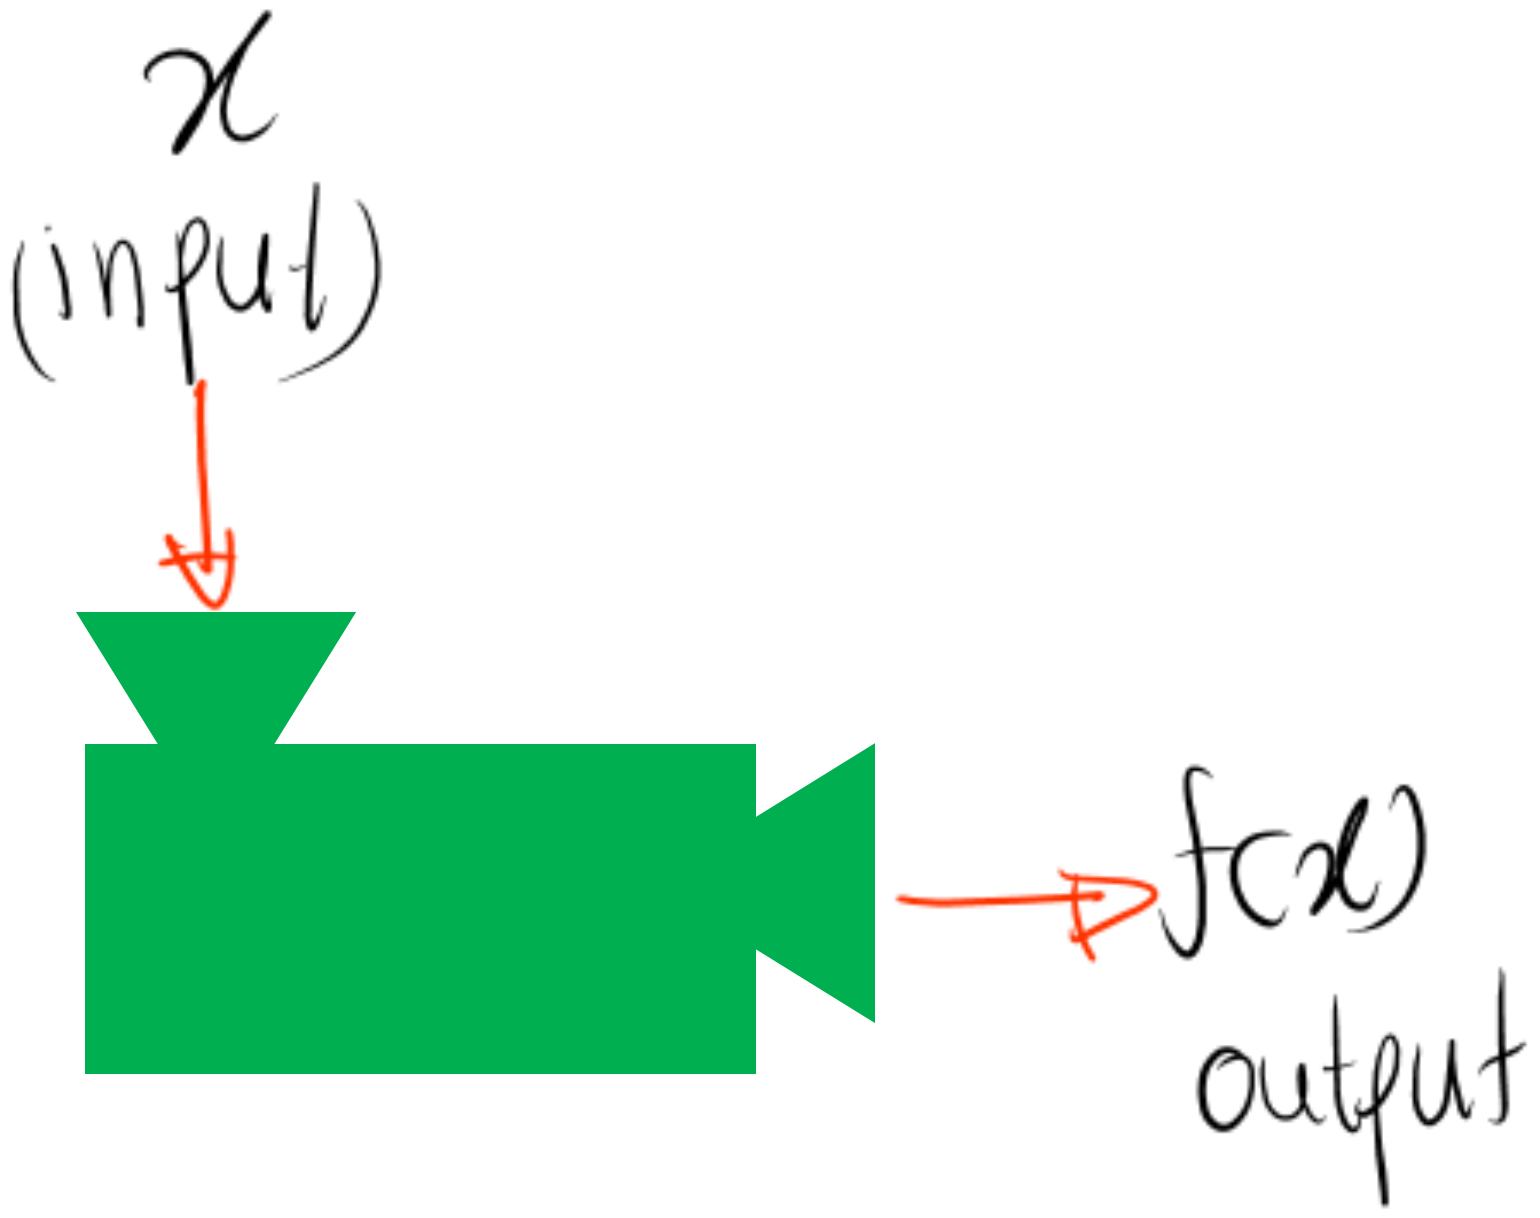
\includegraphics{fig/fig2.png}

If is in the domain of the function then when enters the machine, it's accepted as an input and the machine produces an output according to the rule of the function. Thus we can think of the domain as the set of all possible inputs and the range as the set of all possible outputs.

The graph of also allows us to picture the domain of on the \(x\)-axis and its range on the \(y\)-axis as in Figure \ref{fig:fig4}.

\begin{figure}
\centering
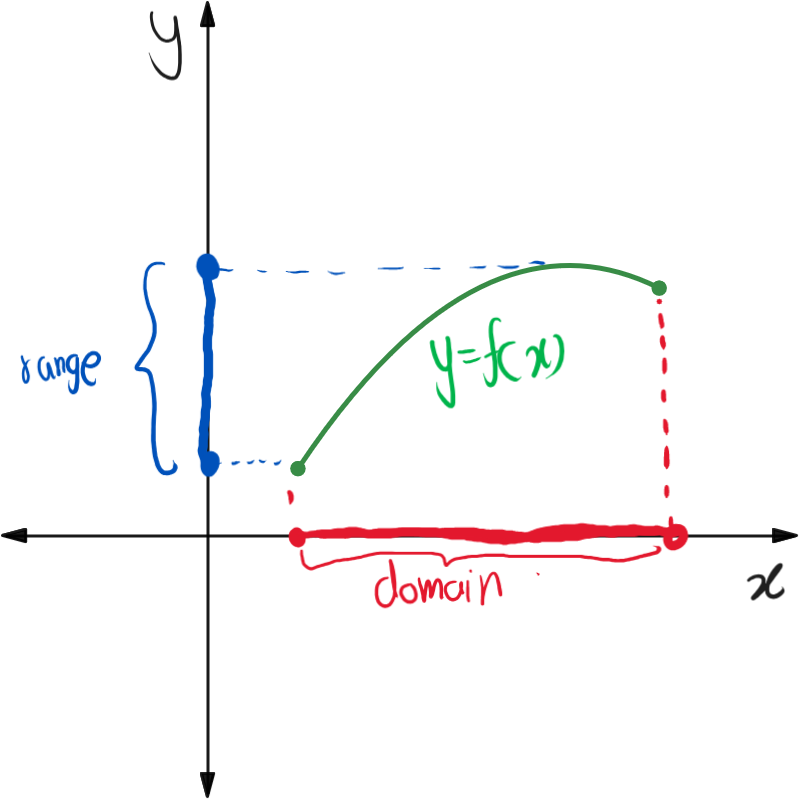
\includegraphics[width=0.5\textwidth,height=\textheight]{fig/fig4.png}
\caption{. \label{fig:fig4}}
\end{figure}

\subsubsection{Representing Functions}\label{representing-functions}

The rule describing the function can be represented by a:

\begin{itemize}
\tightlist
\item
  Picture
\end{itemize}

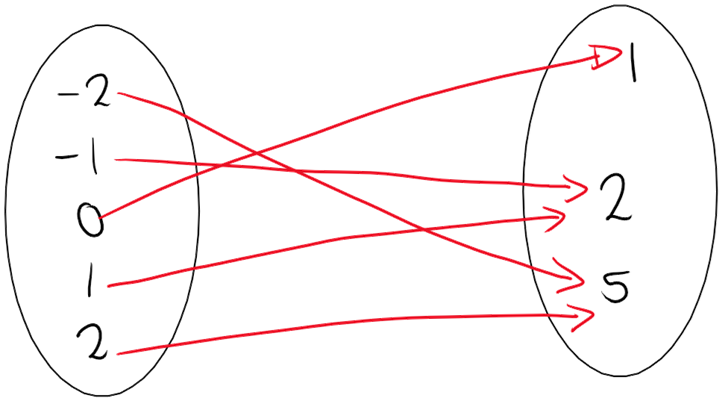
\includegraphics{fig/fig1.png}

\begin{itemize}
\tightlist
\item
  Table
\end{itemize}

\begin{longtable}[]{@{}cc@{}}
\toprule\noalign{}
\(x\) & \(y\) \\
\midrule\noalign{}
\endhead
\bottomrule\noalign{}
\endlastfoot
\(−2\) & \(5\) \\
\(−1\) & \(2\) \\
\(0\) & \(1\) \\
\(1\) & \(2\) \\
\(2\) & \(5\) \\
\end{longtable}

\begin{itemize}
\tightlist
\item
  Formula \(A = \{-2, -1, 0, 1, 2\}, B = \{1, 2, 5\}\) and \(f(x) = x^2 + 1\)
\item
  Cartesian product \(A = \{-2, -1, 0, 1, 2\}, B = \{1, 2, 5\}\) and \(f = \{(-2, 5), (-1, 2), (0, 1), (1, 2), (2, 5)\}\)
\item
  Graph
\end{itemize}

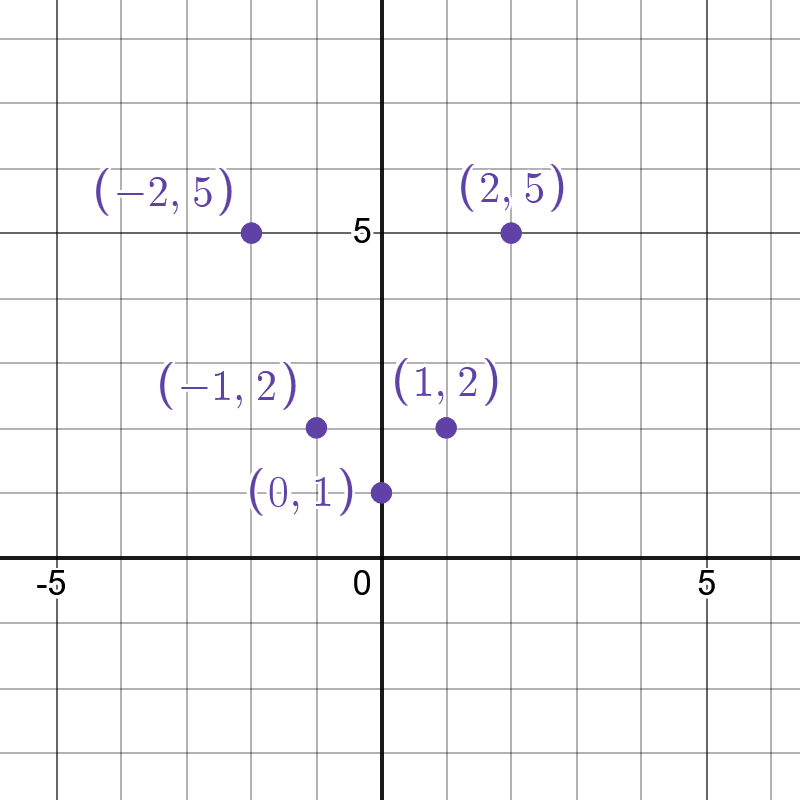
\includegraphics{fig/fig3.png}

\begin{itemize}
\tightlist
\item
  Function Notation
  \[
  f : A \rightarrow B\\
  f(x) = \text{formula}
  \]
  The graph of also allows us to picture the domain of on the \(x\)-axis and its range on the \(y\)-axis as in Figure
\end{itemize}

In this site, unless otherwise specified, the co-domain is the set of real numbers and the domain of a function is the set of real numbers for which the function is defined. We call this the domain convention.

\begin{example}
\protect\hypertarget{exm:unnamed-chunk-2}{}\label{exm:unnamed-chunk-2}

Determine the domain of each function

\begin{enumerate}
\def\labelenumi{\roman{enumi}.}
\tightlist
\item
  \(f(x) = -5x + 1\)
\item
  \(f(x) = \frac{x}{3x^2 - 10x - 8}\)
\item
  \(f(x) = \sqrt{10x - 8}\)
\item
  \(f(x) = \sqrt{3x^2 - 10x + 8}\)
\end{enumerate}

\end{example}

\begin{definition}[Graph of a Function]
\protect\hypertarget{def:unnamed-chunk-3}{}\label{def:unnamed-chunk-3}The graph of a function \(f\) consists of points whose coordinates \((x, y)\) satisfy \(y = f(x)\), for all \(x\) in the domain of \(f\).
\end{definition}

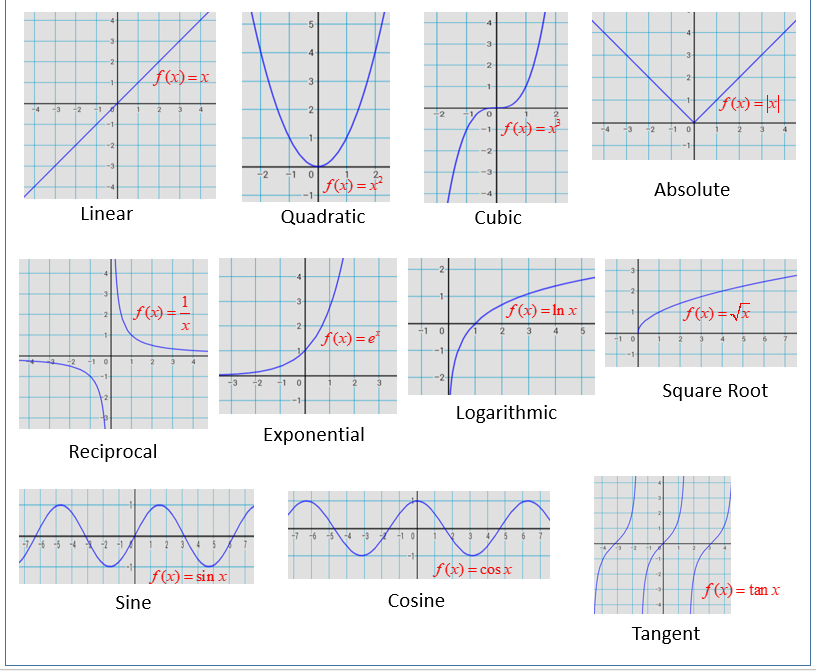
\includegraphics{fig/fig5.png}

\textbf{Vertical Line Test}

A function can only have one output, \(y\), for each unique input, \(x\). If a vertical line intersects a curve on an \(xy\)-plane more than once, then for one value of \(x\) the curve has more than one value of \(y\), and so, the curve does not represent a function.

\begin{example}
\protect\hypertarget{exm:unnamed-chunk-4}{}\label{exm:unnamed-chunk-4}Use the vertical line test to determine when the graph is known.
\end{example}

\begin{figure}
\centering
\includegraphics{https://images.squarespace-cdn.com/content/v1/54905286e4b050812345644c/1668116667931-V2ZJH5WZH4404DKKAVWL/Recap.jpg}
\caption{Resource: images.squarespace-cdn.com}
\end{figure}

\section{Piecewise Defined Functions}\label{piecewise-defined-functions}

A piecewise-defined function (also called a piecewise function) is a function defined by multiple sub-functions, where each sub-function applies to a different interval in the domain.\\
The absolute value function, \(f(x) = |x|\)

\[f(x) = \begin{cases} x & x \ge 0 \\ -x & x < 0 \end{cases}\]
\includesvg{https://upload.wikimedia.org/wikipedia/commons/6/6b/Absolute_value.svg}

\[g(x) = \begin{cases} x^2 & x < 1 \\ -(x - 2)^2 + 5 & x \geq 1 \end{cases}\]
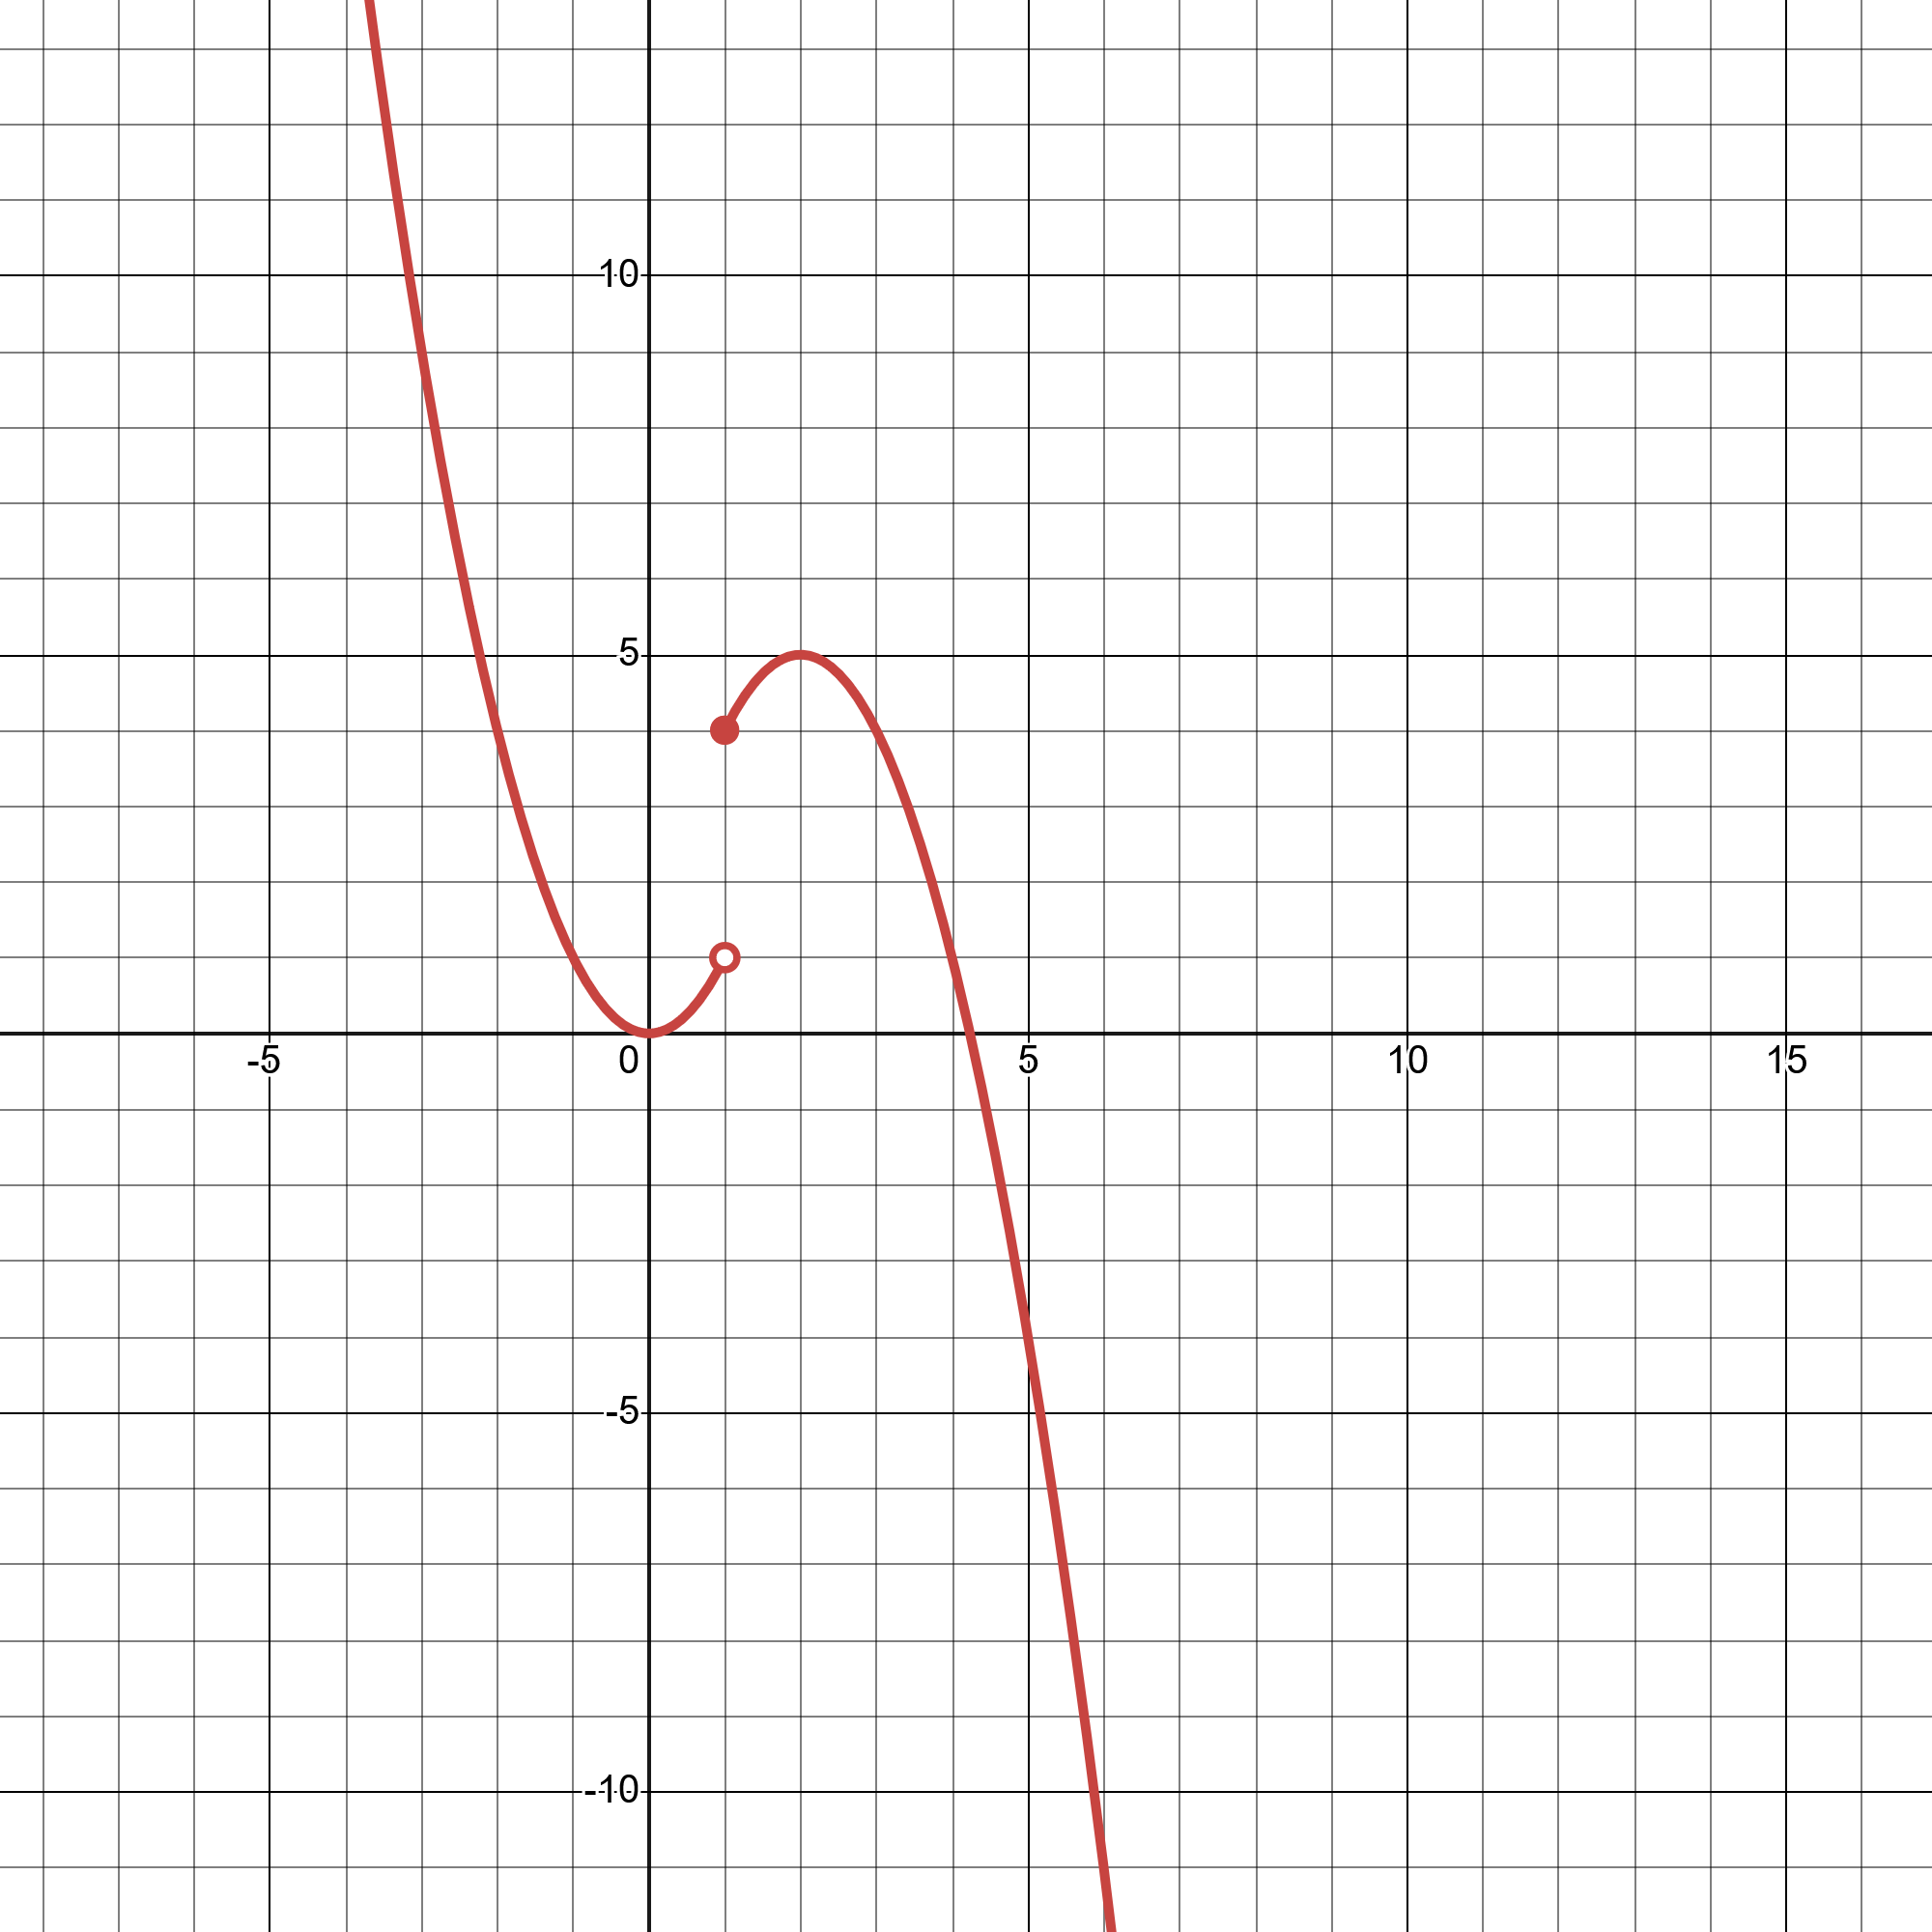
\includegraphics{fig/fig6.png}

\begin{example}
\protect\hypertarget{exm:unnamed-chunk-5}{}\label{exm:unnamed-chunk-5}Given that \(f(t) =\begin{cases} 2t & t \le 1 \\ 2t + 1 & 1 < t < 3 \\ -2t + 2 & t \ge 3 \end{cases}\)

Compute \(f(0), f(1), f(2), f(3), f(5)\)
\end{example}

\section{Combining Functions}\label{combining-functions}

If we are given two functions \(f(x)\) and \(g(x)\), is it possible to combine them in some way? YES!

\begin{enumerate}
\def\labelenumi{\arabic{enumi}.}
\tightlist
\item
  Combining functions arithmetically

  \begin{itemize}
  \tightlist
  \item
    Addition of functions \((f + g)(x) = f(x) + g(x)\)
  \item
    Subtraction of functions \((f - g)(x) = f(x) - g(x)\)
  \item
    Multiplication of functions \((fg)(x) = (f(x)) \cdot (g(x))\)
  \item
    Division of functions \((f/g)(x) = \frac{f(x)}{g(x)}\). BE CAREFUL! We can do this only when \(g(x) \neq 0\)
  \end{itemize}
\item
  Composition of functions \((g \circ f)(x) = g(f(x))\)
\end{enumerate}

\begin{figure}
\centering
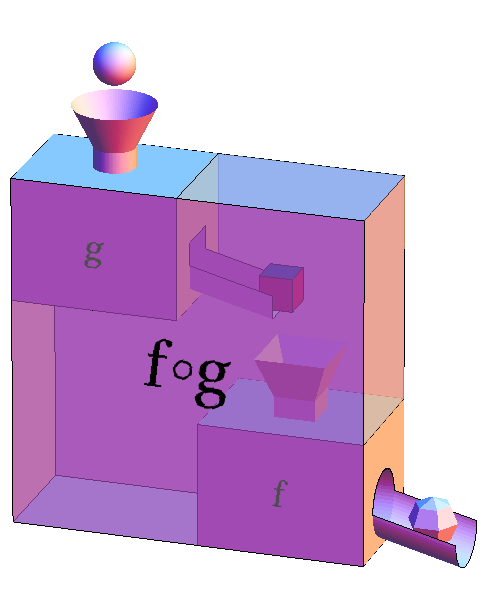
\includegraphics{fig/fig12.png}
\caption{Resource: Mathe Insight}
\end{figure}

\begin{example}
\protect\hypertarget{exm:unnamed-chunk-6}{}\label{exm:unnamed-chunk-6}

Given that \(f(x) = x^2 + 5x + 6\) and \(g(x) = \sqrt{x}\), find

\begin{enumerate}
\def\labelenumi{\roman{enumi}.}
\tightlist
\item
  \(f + g\)
\item
  \(f - g\)
\item
  \(fg\)
\item
  \(\frac{f}{g}\)
\item
  \(f \circ g\) and \(g \circ f\)
\end{enumerate}

\end{example}

\section{Inverse Functions}\label{inverse-functions}

\begin{itemize}
\tightlist
\item
  QUESTION: Suppose you are given a function \(y = f(x)\). For each value of \(y\), can you find a corresponding value of \(x\)?\\
\item
  ANSWER: Maybe\ldots{} depending on the actual \(f(x)\) given.\\
  If we could, we have to solve the equation \(y = f(x)\) for \(x\). The solution is called the ``inverse function of \(f\)'', and denoted by notation \(f^{-1}\).
\end{itemize}

\includegraphics{https://s3-us-west-2.amazonaws.com/courses-images-archive-read-only/wp-content/uploads/sites/924/2015/11/25200955/CNX_Precalc_Figure_01_07_0032.jpg}
\includegraphics{https://upload.wikimedia.org/wikipedia/commons/f/fe/Fruit_function_and_inverse.PNG}

\begin{definition}
\protect\hypertarget{def:unnamed-chunk-7}{}\label{def:unnamed-chunk-7}Let \(f\) be a function with domain \(D\) and range \(R\). Then the function \(g\) with domain \(R\) and range \(D\) is the inverse of \(f\) if

\[
g \circ f(x) = x \quad \forall x \in D
\]
and

\[
f \circ g(x) = x \quad \forall x \in R
\]

If \(g\) is the inverse of \(f\), we denote it by \(g = f^{-1}\).
\end{definition}

\begin{example}
\protect\hypertarget{exm:unnamed-chunk-8}{}\label{exm:unnamed-chunk-8}Given that \(f(x) = \frac{2x + 8}{5}\), find \(f^{-1}\), and verify that the function you found is the inverse of \(f\).
\end{example}

\chapter{Limits and Continuity}\label{limits-and-continuity}

\section{The Limit of a Function}\label{the-limit-of-a-function}

Intuitive definition of limit

\begin{definition}[Left Limit]
\protect\hypertarget{def:unnamed-chunk-9}{}\label{def:unnamed-chunk-9}We write \(\lim_{{x \to c^-}} f(x) = L\) if the number \(f(x)\) (the function height) keeps getting close to \(L\) as \(x\) approaches \(c\) from the left.
\end{definition}

\begin{definition}[Right Limit]
\protect\hypertarget{def:unnamed-chunk-10}{}\label{def:unnamed-chunk-10}We write \(\lim_{{x \to c^+}} f(x) = L\) if the number \(f(x)\) (the function height) keeps getting close to \(L\) as \(x\) approaches \(c\) from the right.
\}

Left Limit and Right Limit are called one-sided limits.
\end{definition}

\begin{definition}[Two-sided Limit]
\protect\hypertarget{def:unnamed-chunk-11}{}\label{def:unnamed-chunk-11}We write

\(\lim_{{x \to c}} f(x) = L\)

if the number \(f(x)\) (the function height) keeps getting close to the
same value \(L\) as \(x\) approaches \(c\) from either direction.
\end{definition}

\begin{theorem}
\protect\hypertarget{thm:unnamed-chunk-12}{}\label{thm:unnamed-chunk-12}The two-sided limit

\[\lim_{{x \to c}} f(x)\]

exists if and only if the two one-sided limits

\[\lim_{{x \to c^-}} f(x) \quad \text{and} \quad \lim_{{x \to c^+}} f(x)\]

both exist and are equal. Furthermore, if

\[\lim_{{x \to c^-}} f(x) = L \quad \text{and} \quad \lim_{{x \to c^+}} f(x) = L\]

then

\[\lim_{{x \to c}} f(x) = L.\]
\end{theorem}

\begin{example}[Evaluating limits using a graph]
\protect\hypertarget{exm:ex315}{}\label{exm:ex315}For each of the following functions, write down the left limit, right limit, two-sided limit, and the function value at the given point. If any limit is undefined, write "UND".

\begin{itemize}
\tightlist
\item
  at \(x = 4\)
\end{itemize}

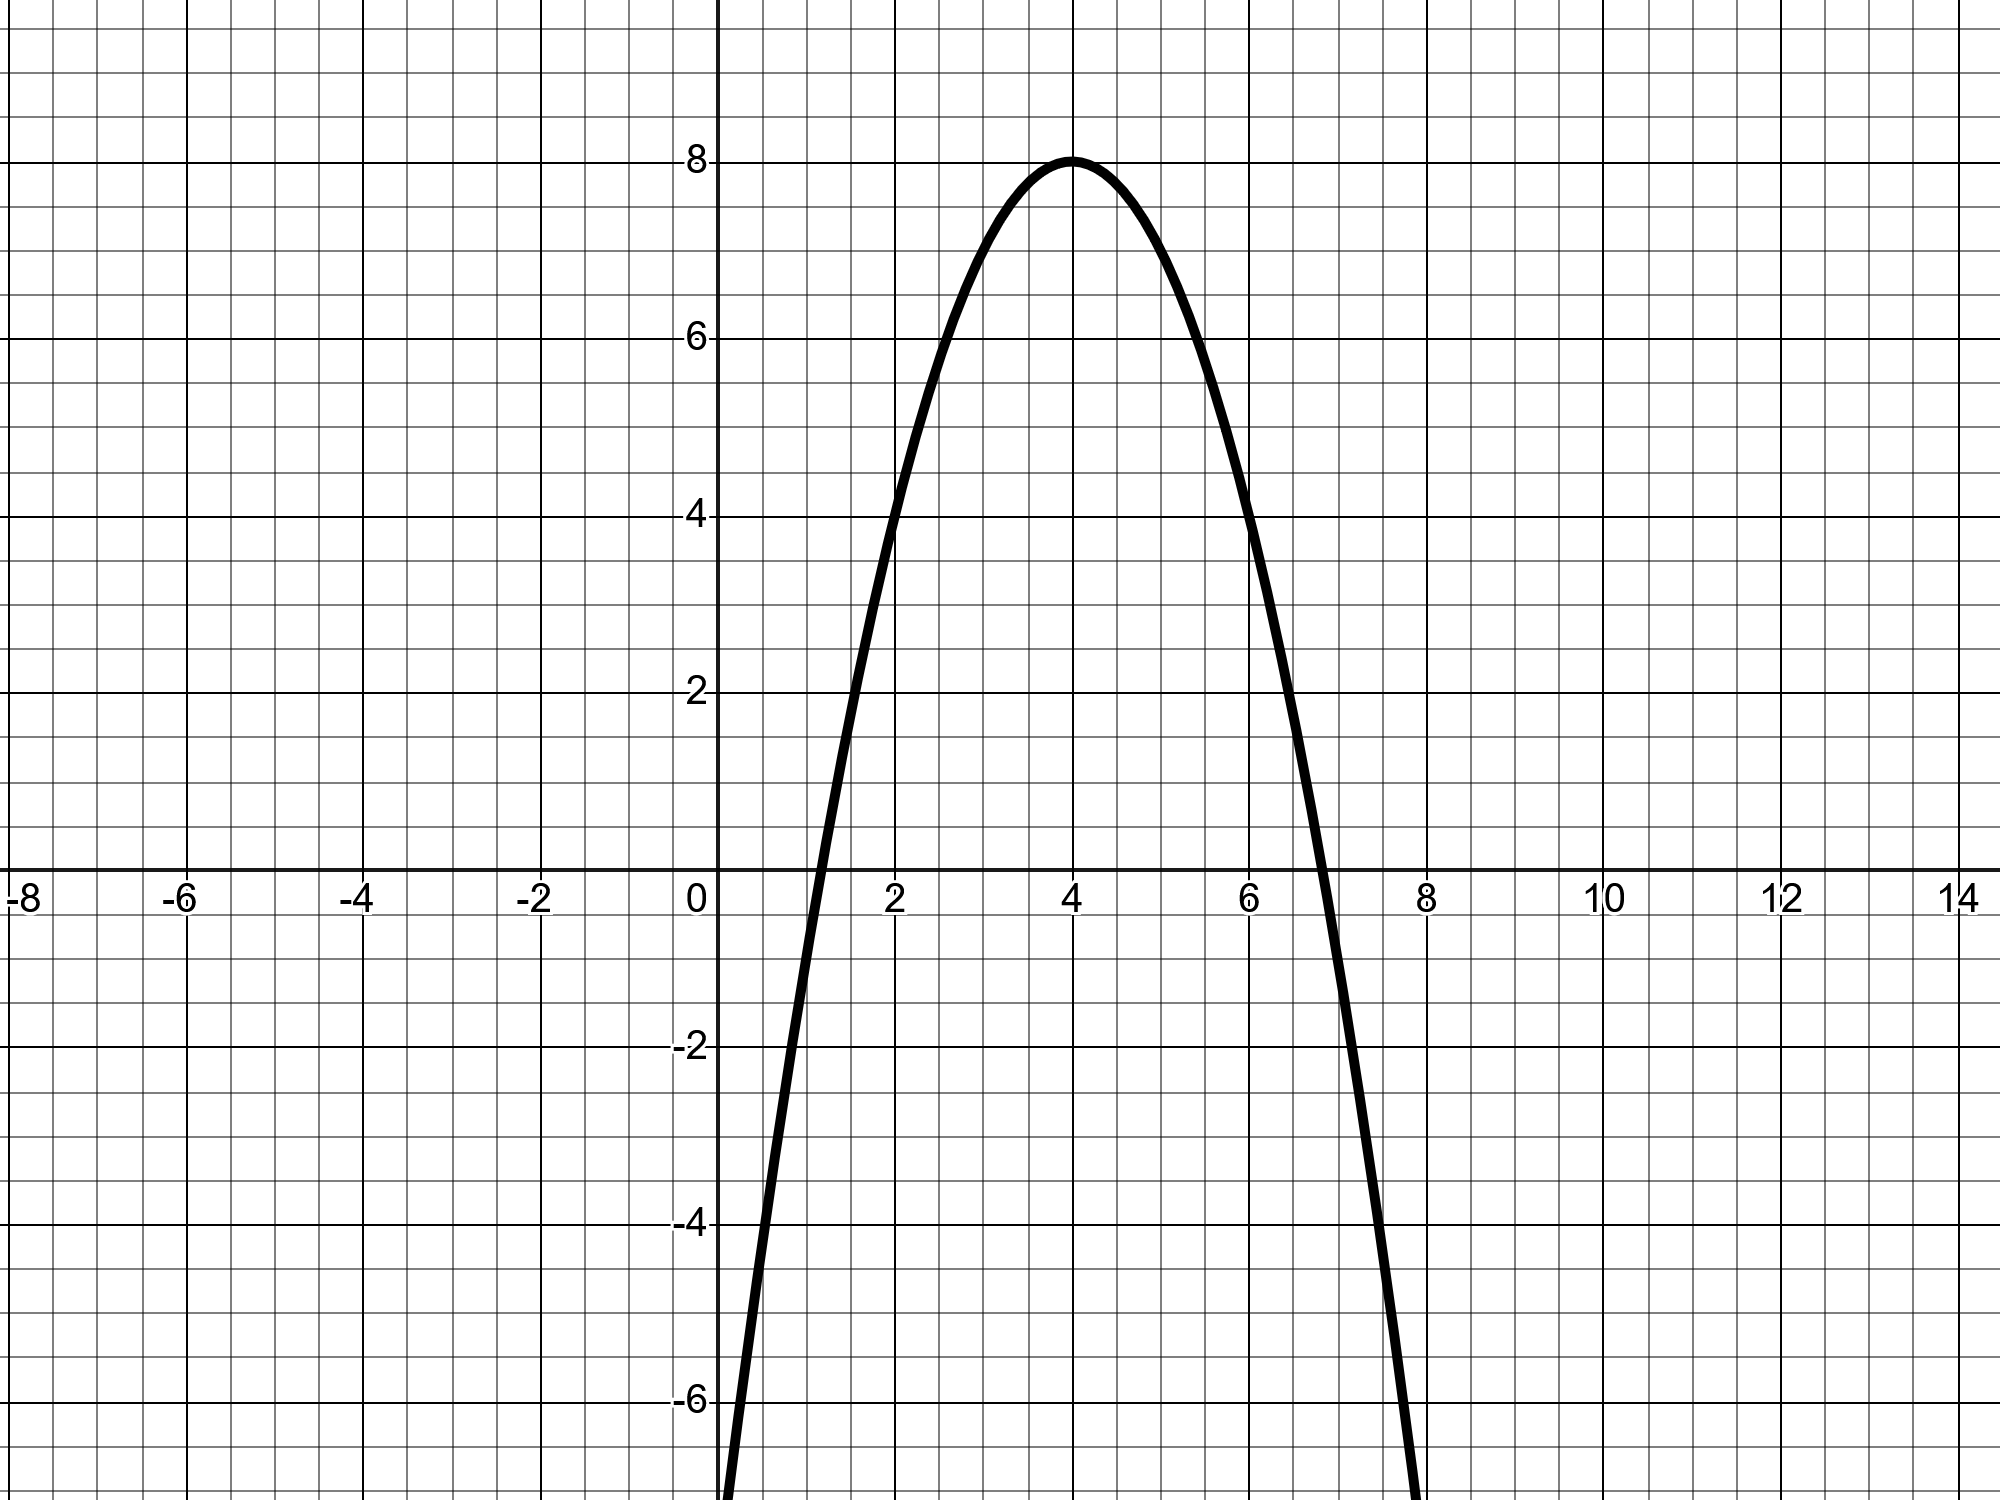
\includegraphics{fig/fig7.png}

\begin{itemize}
\tightlist
\item
  at \(x = 3\)
\end{itemize}

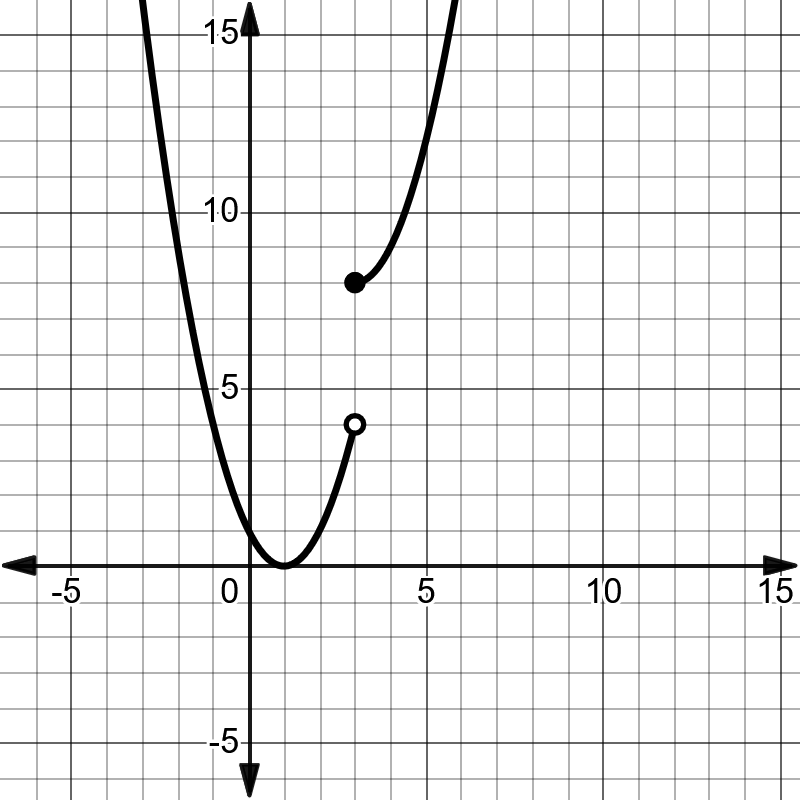
\includegraphics{fig/fig8.png}

\begin{itemize}
\tightlist
\item
  at \(x = -2\)
\end{itemize}

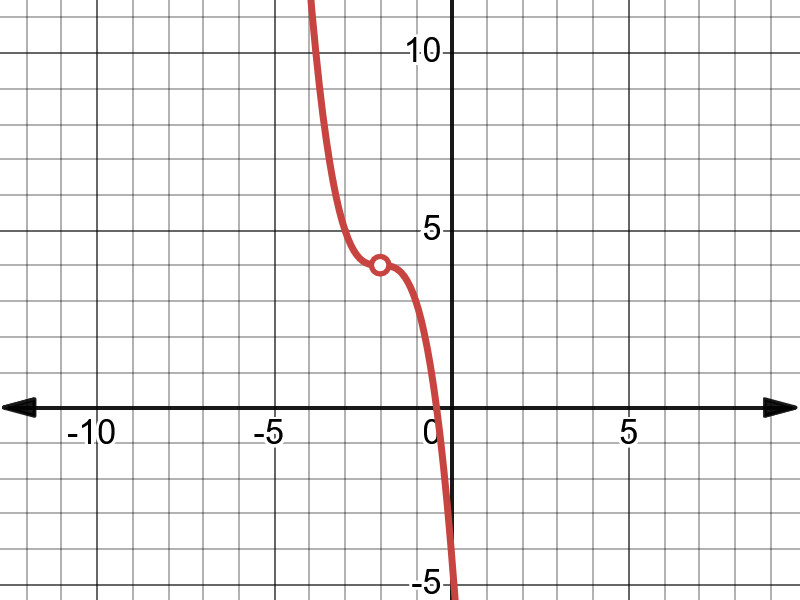
\includegraphics{fig/fig9.png}

\begin{itemize}
\tightlist
\item
  at \(x = 3\)
\end{itemize}

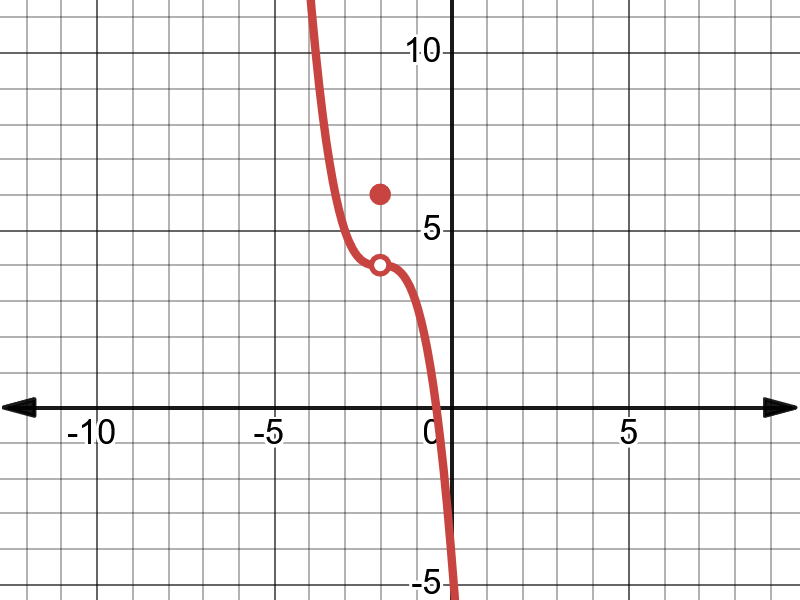
\includegraphics{fig/fig10.png}
\end{example}

\begin{remark}

In Example @ref\{exm:ex315\}

\begin{itemize}
\item
  part (a), you can observe that the limit (two-sided limit) at \(x = 2\) is equal to the function value at that point.
\item
  In part (d), you can observe that the limit (two-sided
  limit) at \(x = 3\) is different from the function value at that point.
\item
  In general, there is no connection between the limit of a function at a point (\(\lim_{{x \to c}} f(x)\)) and the value of the function (\(f(c)\))
  at that point.
\end{itemize}

\end{remark}

\begin{example}
\protect\hypertarget{exm:unnamed-chunk-14}{}\label{exm:unnamed-chunk-14}\leavevmode

\begin{longtable}[]{@{}ll@{}}
\toprule\noalign{}
x & f(x) \\
\midrule\noalign{}
\endhead
\bottomrule\noalign{}
\endlastfoot
-0.05 & 2.0025 \\
-0.25 & 2.0625 \\
-0.01 & 2.0001 \\
-0.001 & 2.000001 \\
0.001 & 2.000001 \\
0.01 & 2.0001 \\
0.25 & 2.0625 \\
0.5 & 2.25 \\
\end{longtable}

Observing the table, we can say there is a good
chance that

\[\lim_{{x \to 0}} f(x) = 2.\]

One cannot use a table to calculate the limit exactly (Why?).

\end{example}

\begin{example}
\protect\hypertarget{exm:unnamed-chunk-15}{}\label{exm:unnamed-chunk-15}The following figure shows the graph of
\(f(x) = \sin\left(\frac{1}{x}\right)\). Observe that

\[\lim_{{x \to 0}} \sin\left(\frac{1}{x}\right)\]

is undefined.
\end{example}

\begin{figure}
\centering
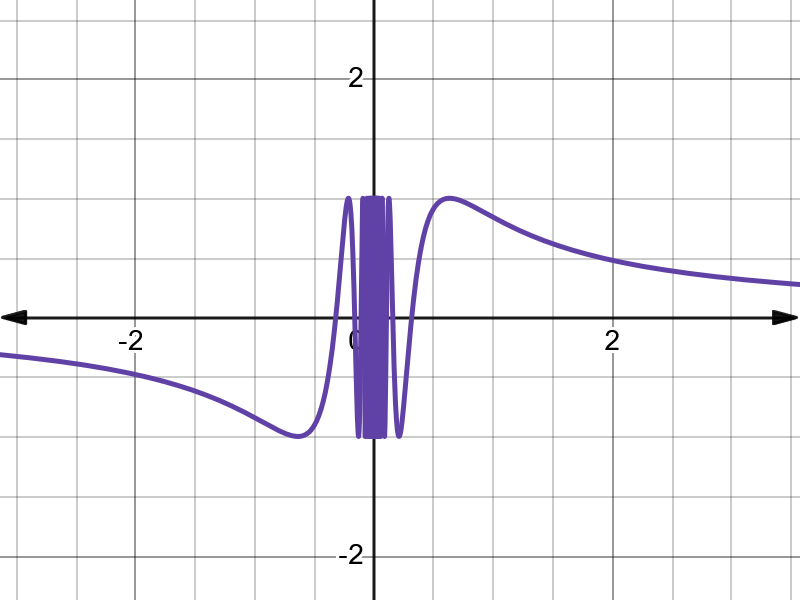
\includegraphics{fig/fig11.png}
\caption{Graph of \(f(x) =\sin\left(\frac{1}{x}\right)\).}
\end{figure}

The graph is better than the table when we use Definition 3.1. In this
course, we stick with Definition 3.1. It's not rigorous enough; you will learn the formal \(\epsilon - \delta\) definition listed below in advanced math classes.

\begin{definition}
\protect\hypertarget{def:unnamed-chunk-16}{}\label{def:unnamed-chunk-16}Let \(f: \mathbb{R} \to \mathbb{R}\) and
\(L \in \mathbb{R}\). We say that the limit of \(f\) at \(c\) is \(L\) and
denote it by

\[\lim_{{x \to c}} f(x) = L,\]

if for each \(\epsilon > 0\), there exists \(\delta > 0\) such that:

\[|x - c| < \delta \Rightarrow |f(x) - L| < \epsilon.\]
\end{definition}

\section{Continuity}\label{continuity}

In the most basic sense, a continuous function can be sketched in one
continuous stroke without lifting a pen or pencil. We would need to lift our pencil in drawing a function because it has a jump or hole in its graph. If there is a jump or hole in the graph, at that point, either the limit or function value is undefined, or they take different values. This leads to the following definition.

\begin{definition}[Continuity at a point]
\protect\hypertarget{def:unnamed-chunk-17}{}\label{def:unnamed-chunk-17}We say a function is continuous at a point \(x = c\), if the number \(f(x)\) (the function height) keeps getting close to \(f(c)\) as \(x\) approaches \(c\) from either direction. A function that is not continuous at \(c\) is said to have a discontinuity at that point.
\end{definition}

Following theorem is straightforward.

\begin{theorem}[Continuity theorem I]
\protect\hypertarget{thm:unnamed-chunk-18}{}\label{thm:unnamed-chunk-18}

A function \(f\) is continuous
at a point \(x = c\) if the following conditions are satisfied:

\begin{enumerate}
\def\labelenumi{\arabic{enumi}.}
\item
  \(f(c)\) is defined;
\item
  \(\lim_{{x \to c}} f(x)\) is defined;
\item
  \(\lim_{{x \to c}} f(x) = f(c)\).
\end{enumerate}

\end{theorem}

\begin{example}
\protect\hypertarget{exm:unnamed-chunk-19}{}\label{exm:unnamed-chunk-19}For each of the following functions, state whether the function is continuous at the given point. If not, state which condition of continuity is broken at that point.

\begin{itemize}
\tightlist
\item
  at \(x = 4\)
\end{itemize}

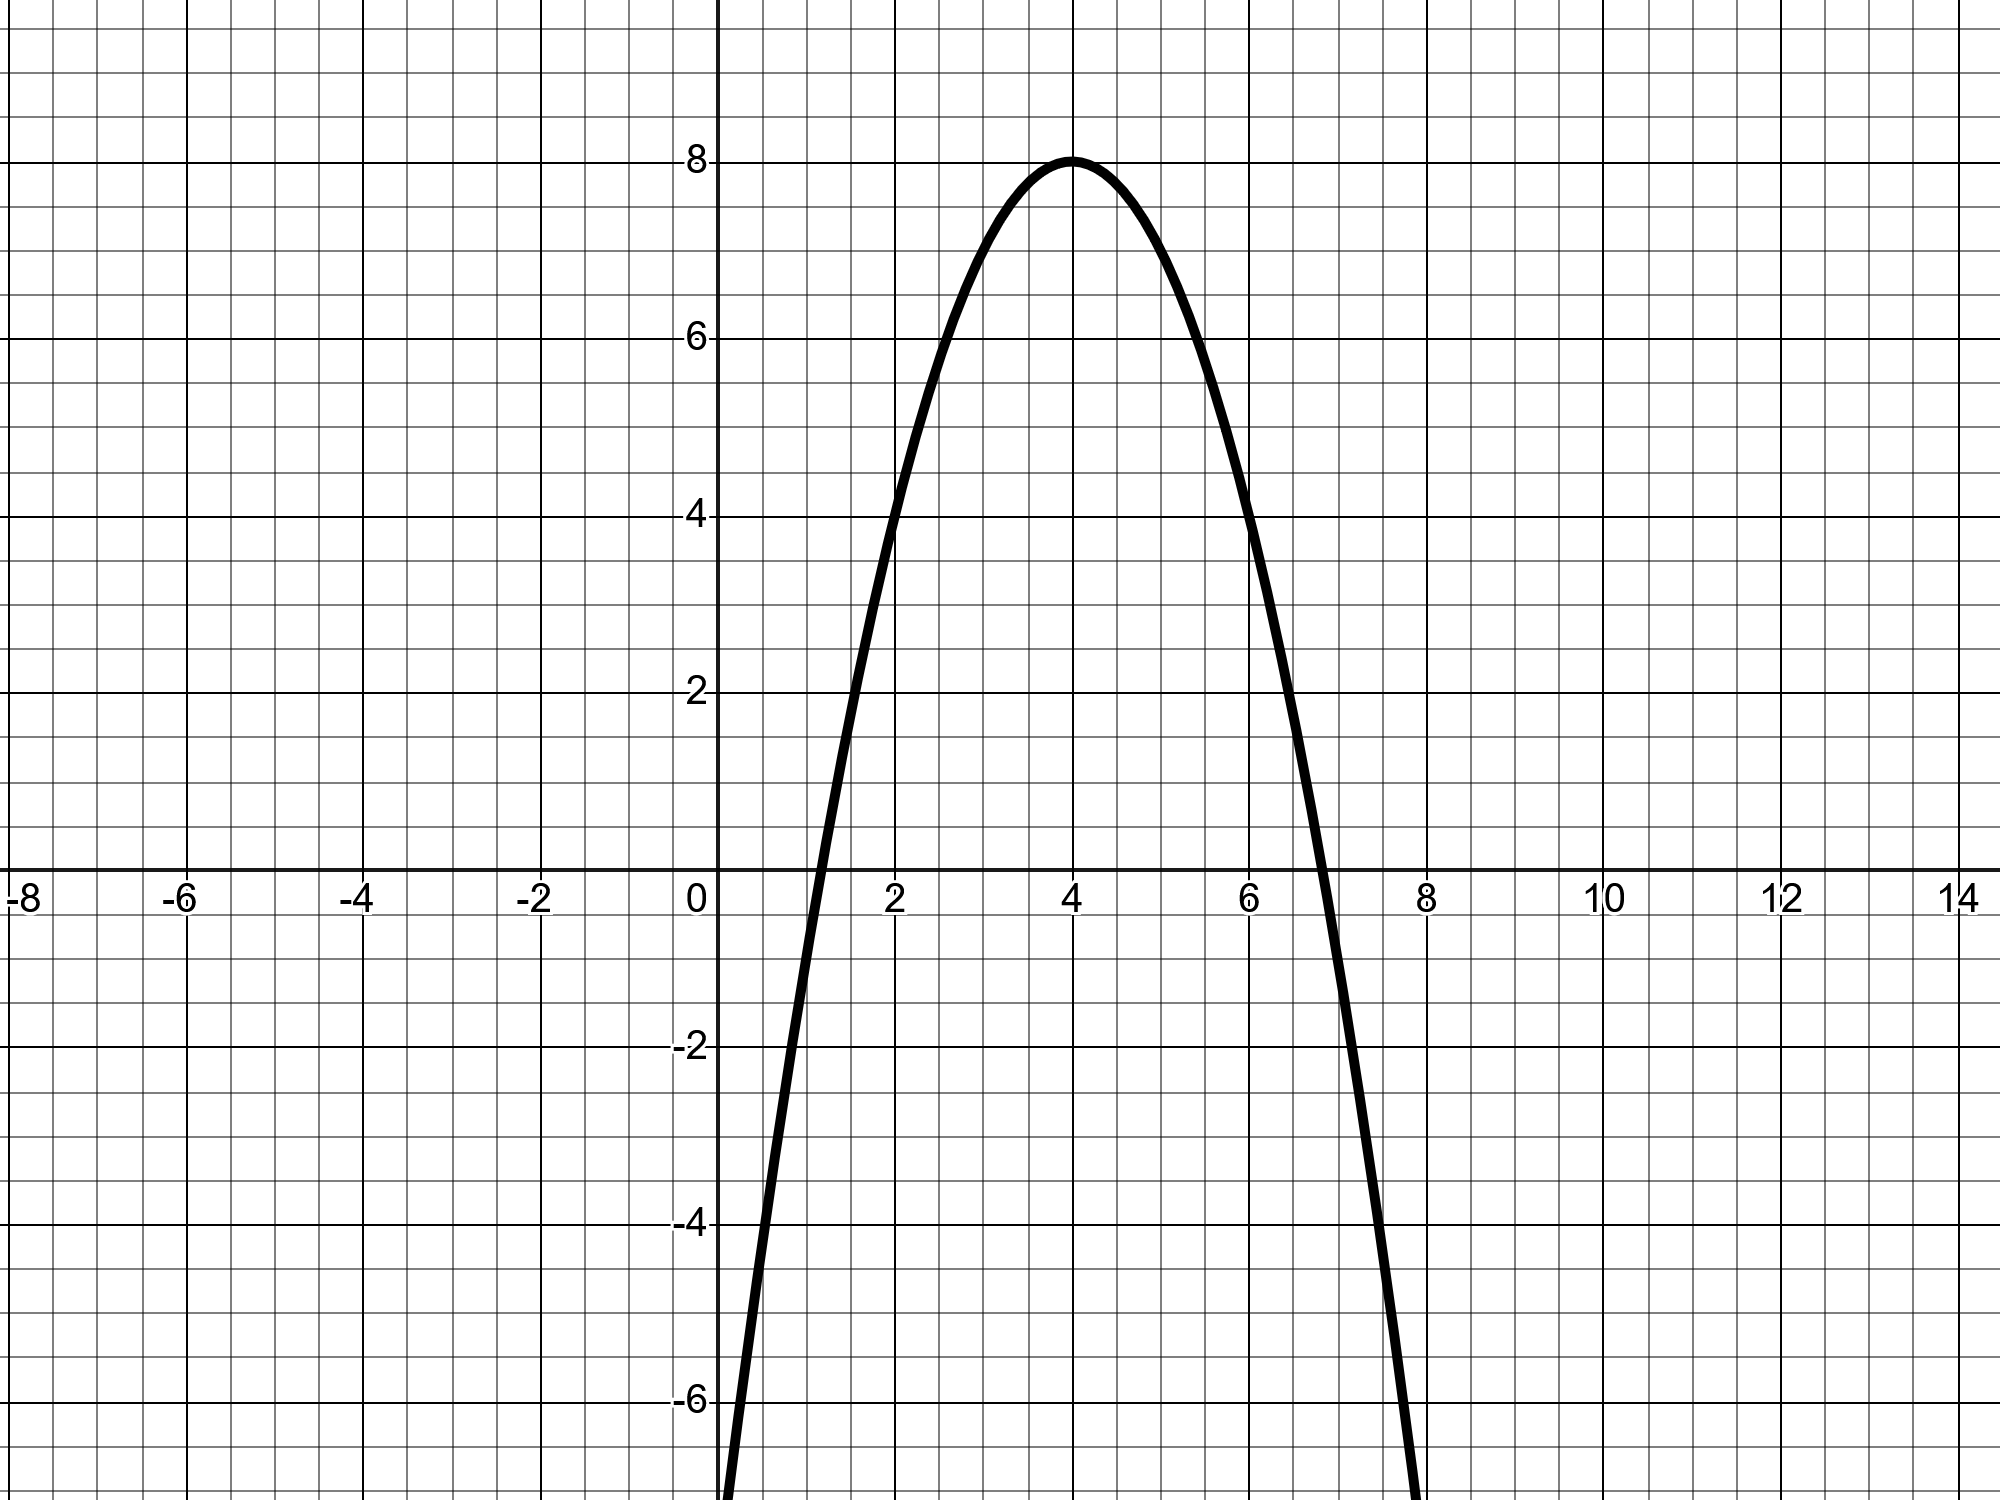
\includegraphics{fig/fig7.png}

\begin{itemize}
\tightlist
\item
  at \(x = 3\)
\end{itemize}

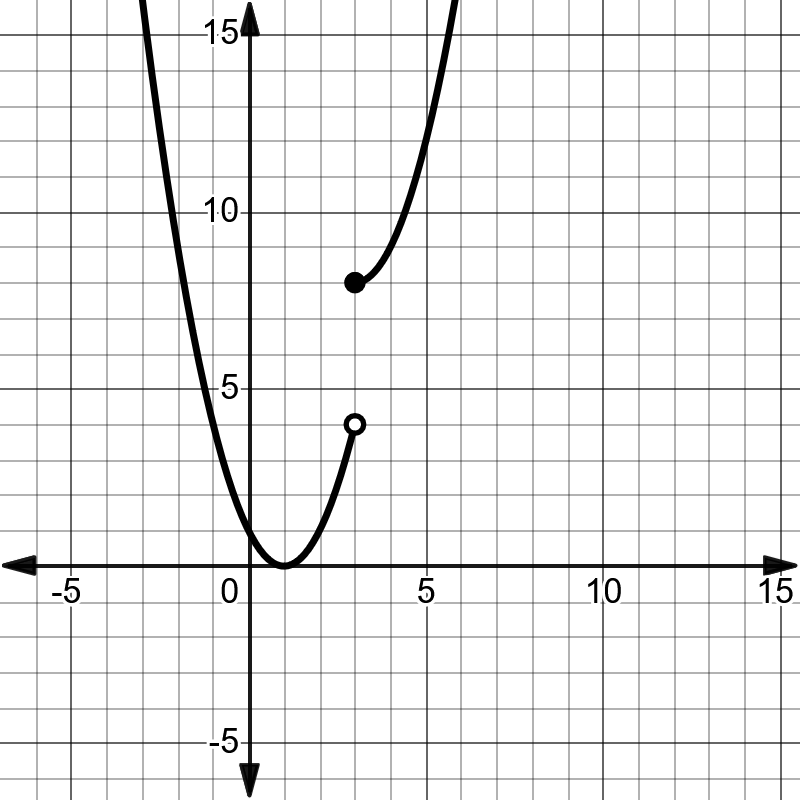
\includegraphics{fig/fig8.png}

\begin{itemize}
\tightlist
\item
  at \(x = -2\)
\end{itemize}

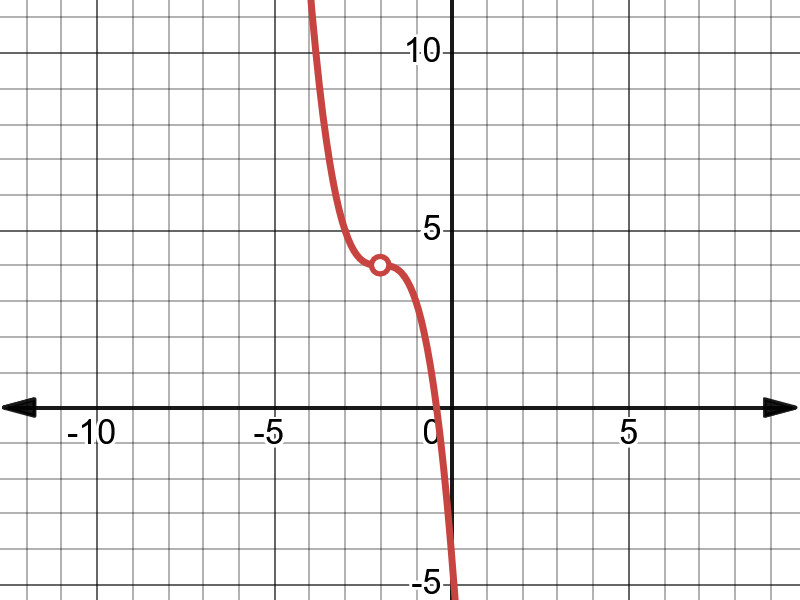
\includegraphics{fig/fig9.png}

\begin{itemize}
\tightlist
\item
  at \(x = 3\)
\end{itemize}

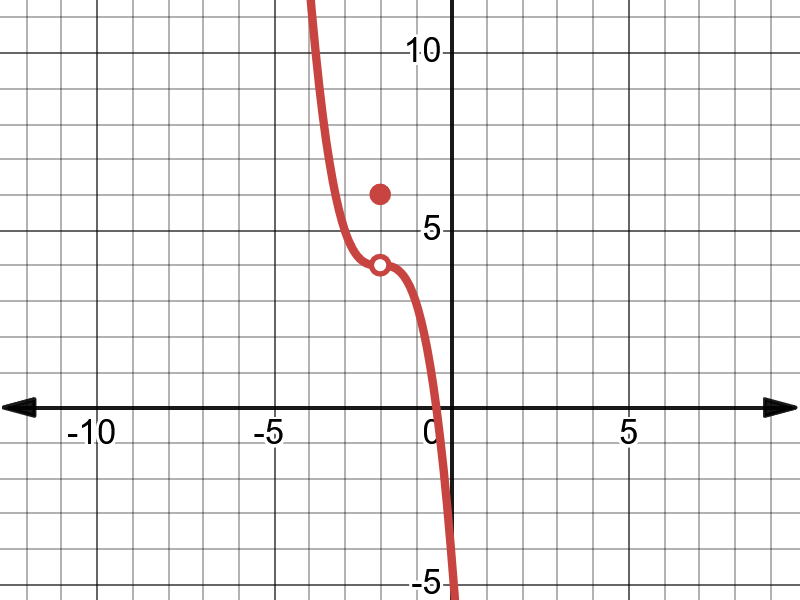
\includegraphics{fig/fig10.png}
\end{example}

\begin{definition}[Continuity of a function]
\protect\hypertarget{def:unnamed-chunk-20}{}\label{def:unnamed-chunk-20}A function is
\textbf{continuous on a set} \(X\) if it is continuous at every point of \(X\).
\end{definition}

\begin{definition}
\protect\hypertarget{def:unnamed-chunk-21}{}\label{def:unnamed-chunk-21}Let \(f: \mathbb{R} \to \mathbb{R}\) and
\(c \in \mathbb{R}\). \(f\) is continuous at \(c\) if for each \(\epsilon > 0\),
there exists \(\delta > 0\) such that:

\[|x - c| < \delta \Rightarrow |f(x) - f(c)| < \epsilon.\]
\end{definition}

\section{Algebraic computation of limits}\label{algebraic-computation-of-limits}

\begin{theorem}[Basic properties and rules for limits]
\protect\hypertarget{thm:unnamed-chunk-22}{}\label{thm:unnamed-chunk-22}For any real number \(c\), suppose that functions \(f\) and \(g\) both have
limits at \(x = c\).

\begin{itemize}
\item
  \textbf{Constant rule:} \(\lim_{{x \to c}} k = k\).
\item
  \textbf{Multiple rule:}
  \(\lim_{{x \to c}} [kf(x)] = k \lim_{{x \to c}} f(x)\) for any
  constant \(k\).
\item
  \textbf{Sum rule:}
  \(\lim_{{x \to c}} [f(x) + g(x)] = \lim_{{x \to c}} f(x) + \lim_{{x \to c}} g(x)\).
\item
  \textbf{Difference rule:}
  \(\lim_{{x \to c}} [f(x) - g(x)] = \lim_{{x \to c}} f(x) - \lim_{{x \to c}} g(x)\).
\item
  \textbf{Product rule:}
  \(\lim_{{x \to c}} [f(x) g(x)] = [\lim_{{x \to c}} f(x)][\lim_{{x \to c}} g(x)]\).
\item
  \textbf{Quotient rule:}
  \(\lim_{{x \to c}} \frac{f(x)}{g(x)} = \frac{\lim_{{x \to c}} f(x)}{\lim_{{x \to c}} g(x)}\)
  if \(\lim_{{x \to c}} g(x) \neq 0\).
\item
  \textbf{Power rule:}
  \(\lim_{{x \to c}} [f(x)]^n = [\lim_{{x \to c}} f(x)]^n\).
\end{itemize}

By using the \(\epsilon - \delta\) definition of continuity and the above
theorem, we can establish the continuity of basic functions.
\end{theorem}

\begin{example}
\protect\hypertarget{exm:unnamed-chunk-23}{}\label{exm:unnamed-chunk-23}Prove that \(f(x) = x\) is continuous on the set of
real numbers.
\end{example}

\begin{proof}
For any \(c \in \mathbb{R}\) and \(\epsilon > 0\) let
\(\delta = \epsilon\).

\[|x - c| < \delta \Rightarrow |x - c| < \epsilon \Rightarrow |f(x) - f(c)| < \epsilon\]
\end{proof}

\begin{theorem}[Continuity theorem II]
\protect\hypertarget{thm:unnamed-chunk-25}{}\label{thm:unnamed-chunk-25}If \(f\) is a polynomial function, a rational function, a trigonometric
function, a trigonometric inverse function, an exponential function, or
a logarithmic function, then \(f\) is continuous at any number \(x = c\) for which \(f(c)\) is defined.
\end{theorem}

\begin{proof}
Omitted
\end{proof}

\begin{remark}
We can plug in the value to find the limit only if we
know that the function is continuous at that point.
\end{remark}

\begin{example}
\protect\hypertarget{exm:unnamed-chunk-28}{}\label{exm:unnamed-chunk-28}

Evaluate each of the following limits:

\begin{enumerate}
\def\labelenumi{\roman{enumi})}
\tightlist
\item
  \(\lim_{{x \to \frac{\pi}{6}}} \sin(x)\)
\item
  \(\lim_{{x \to \frac{\pi}{6}}} \cos(x)\)
\item
  \(\lim_{{x \to -\frac{\pi}{4}}} \sin(x)\)
\item
  \(\lim_{{x \to 2}} x\)
\item
  \(\lim_{{x \to \frac{\pi}{4}}} [\sin(x) + 2x + 3]\)
\item
  \(\lim_{{x \to \frac{\sqrt{3}}{2}}} [\sin^{-1}(x) + \cos^{-1}(x)]\)
\item
  \(\lim_{{x \to 2}} [2x^2 + 5x + 6]\)
\item
  \(\lim_{{x \to 6}} [\ln(x) + e^x]\)
\item
  \(\lim_{{x \to \frac{\pi}{6}}} \tan(x)\)
\item
  \(\lim_{{x \to 2}} [2x^2 + 5x + 6]\)
\item
  \(\lim_{{x \to \frac{\pi}{4}}} \frac{\sin(x) + \cos(x)}{\sin(x) \cos(x)}\)
\end{enumerate}

\end{example}

\section{\texorpdfstring{Limits involving indeterminate forms \(\frac{0}{0}\)}{Limits involving indeterminate forms \textbackslash frac\{0\}\{0\}}}\label{limits-involving-indeterminate-forms-frac00}

\textbf{Rational functions}

Evaluate \(\lim_{{x \to 5}} \frac{x^2 - 11x + 30}{x^2 - 25}\)

Let us try applying the Quotient rule:

\[\lim_{{x \to 5}} \frac{x^2 - 11x + 30}{x^2 - 25} = \frac{\lim_{{x \to 5}} [x^2 - 11x + 30]}{\lim_{{x \to 5}} [x^2 - 25]} = \frac{25 - 55 + 30}{25 - 25} = \frac{0}{0}\]

The denominator (namely \(\lim_{{x \to 5}} [x^2 - 25]\)) is zero;
therefore, we cannot use the Quotient rule here.

\begin{remark}

\emph{(Indeterminate form)} In calculus and other branches of
mathematical analysis, an \textbf{indeterminate form} is an algebraic
expression obtained in the context of limits. Limits involving algebraic operations are often performed by replacing expressions by their limits;
if the expression obtained after this substitution does not give enough
information to determine the original limit, it is known as an
indeterminate form. \(\frac{0}{0}\) is one of the indeterminate forms you
will encounter in calculus 1.

Let us examine a method that can be used to go around this problem. We
want to evaluate \(\lim_{{x \to 5}} \frac{x^2 - 11x + 30}{x^2 - 25}\).

Set \(f(x) = \frac{x^2 - 11x + 30}{x^2 - 25}\) and we are looking for
\(\lim_{{x \to 5}} f(x)\). Let us take a closer look at \(f(x)\):

\[f(x) = \frac{x^2 - 11x + 30}{x^2 - 25} = \frac{(x - 5)(x - 6)}{(x - 5)(x + 5)} = \frac{x - 6}{x + 5} \quad \text{when } x \neq \pm 5\]

Still, 5 is not in the domain of \(f\). Define a new function \(g(x)\) by
\(g(x) = \frac{x - 6}{x + 5}\). Observe that \(g(x)\) is originally defined
as \(\frac{x - 6}{x + 5}\) and 5 is in the domain of \(g(x)\).

Now look at the graphs of \(f(x)\) and \(g(x)\). Observe that \(g(x)\) is
defined and continuous at \(x = 5\). Therefore, we can plug in 5 to get
\(\lim_{{x \to 5}} g(x)\):

\[\lim_{{x \to 5}} g(x) = g(5) = \frac{5 - 6}{5 + 5} = -\frac{1}{10}\]

Of course, the graph of \(f(x)\) has a hole at 5. Therefore, \(f\) is not
continuous at 5. We cannot plug in 5 to get \(\lim_{{x \to 5}} f(x)\), but
comparing the graphs of \(f(x)\) and \(g(x)\), one can observe that:

\[\lim_{{x \to 5}} f(x) = \lim_{{x \to 5}} g(x)\]

Since \(\lim_{{x \to 5}} g(x) = -\frac{1}{10}\), \(\lim_{{x \to 5}} f(x)\)
is also \(-\frac{1}{10}\).

The following summarizes the observations we made. Suppose
\(R(x) = \frac{f(x)}{g(x)}\) and we want to evaluate
\(\lim_{{x \to c}} R(x)\). Use of the quotient rule leads to the
indeterminate form \(\frac{0}{0}\). The following steps might help to go
around this problem:

\begin{enumerate}
\def\labelenumi{\arabic{enumi}.}
\item
  Factor out the numerator and denominator.
\item
  Cancel the common factors.
\item
  Use limits rules to evaluate the limit of the remaining function.
\end{enumerate}

\end{remark}

\section{Limits Involving Infinity}\label{limits-involving-infinity}

\subsection{Infinite Limits}\label{infinite-limits}

It may happen that a function \(f\) does not have a finite limit as \(x \rightarrow c\). When \(\lim _{x \rightarrow c} f(x)\) fails to exist, the function values \(f(x)\) are said to diverge as \(x \rightarrow c\).

\begin{example}
\protect\hypertarget{exm:unnamed-chunk-30}{}\label{exm:unnamed-chunk-30}Consider the function \(f(x)=\frac{1}{x^{2}}\).

\begin{longtable}[]{@{}cc@{}}
\toprule\noalign{}
\(x\) & \(f(x)\) \\
\midrule\noalign{}
\endhead
\bottomrule\noalign{}
\endlastfoot
0.1 & 100 \\
0.01 & 10000 \\
0.001 & \(10^{6}\) \\
0.0001 & \(10^{8}\) \\
0.00001 & \(10^{10}\) \\
\end{longtable}

As \(x \rightarrow 0, f(x) \rightarrow \infty\). The graph of \(f(x)=\frac{1}{x^{2}}\) illustrates this behavior.
\end{example}

\begin{figure}
\centering
\includegraphics{https://cdn.mathpix.com/cropped/2024_12_21_cc496b389b0f492c53b9g-35.jpg?height=660&width=747&top_left_y=857&top_left_x=689}
\caption{Graph of \(f(x)=\frac{1}{x^{2}}\)}
\end{figure}

\begin{definition}
\protect\hypertarget{def:unnamed-chunk-31}{}\label{def:unnamed-chunk-31}A function \(f\) that increases or decreases without bound as \(x\) approaches \(c\) is said to tend to infinity ( \(\infty\) ) at c.~We indicate this behavior by writing:

\[
\lim _{x \rightarrow c} f(x)=\infty \quad \text { or } \quad \lim _{x \rightarrow c} f(x)=-\infty
\]
\end{definition}

\begin{example}
\protect\hypertarget{exm:unnamed-chunk-32}{}\label{exm:unnamed-chunk-32}\[
\lim _{x \rightarrow 0} \frac{1}{x^{2}}=\infty
\]

\[
\lim _{x \rightarrow 0^{-}} \frac{1}{x}=-\infty \quad \text { and } \quad \lim _{x \rightarrow 0^{+}} \frac{1}{x}=\infty
\]
\end{example}

The graph of \(f(x)=\frac{1}{x}\) shows this behavior:

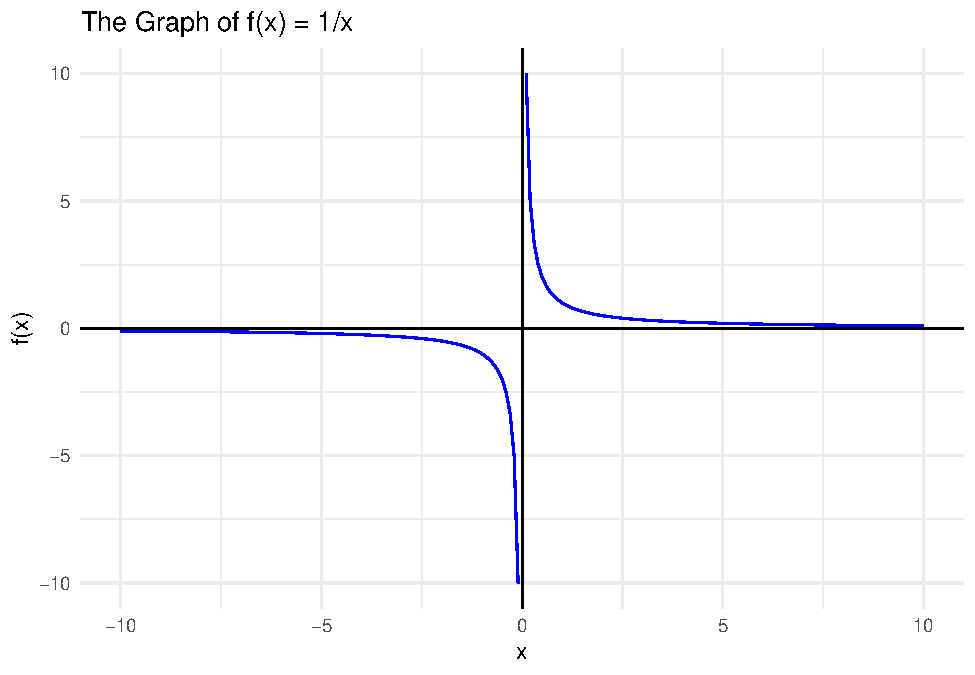
\includegraphics{_main_files/figure-latex/unnamed-chunk-33-1.pdf}

\begin{example}
\protect\hypertarget{exm:unnamed-chunk-34}{}\label{exm:unnamed-chunk-34}Evaluate the limit:

\[
\lim _{x \rightarrow 1}\left(\frac{1}{x^{2}-1}-1\right)
\]

\textbf{Solution}: We begin by substituting \(x=1+h\), where \(h \rightarrow 0\). The expression becomes:

\[
\frac{1}{(1+h)^{2}-1}-1
\]

Expanding \((1+h)^{2}\) :

\[
(1+h)^{2}-1=2 h+h^{2}
\]

So, the expression becomes:

\[
\frac{1}{2 h+h^{2}}-1=\frac{1-\left(2 h+h^{2}\right)}{2 h+h^{2}}=\frac{1-2 h-h^{2}}{2 h+h^{2}}
\]

One-Sided Limits: As \(h \rightarrow 0\) :

\begin{itemize}
\tightlist
\item
  For \(h \rightarrow 0^{+}\)(approaching from the right):
\end{itemize}

For \(h>0\), we analyze the expression \(\frac{1}{2 h+h^{2}}\). Since \(h\) is positive and small, the term \(h^{2}\) is negligible compared to \(2 h\), so the expression behaves similarly to \(\frac{1}{2 h}\).

As \(h \rightarrow 0^{+}, 2 h\) becomes very small, and the reciprocal \(\frac{1}{2 h}\) grows without bound towards \(+\infty\).
Thus, the limit from the right is \(+\infty\).

\begin{itemize}
\tightlist
\item
  For \(h \rightarrow 0^{-}\)(approaching from the left):
\end{itemize}

For \(h<0\), the expression \(\frac{1}{2 h+h^{2}}\) behaves similarly to \(\frac{1}{2 h}\), but since \(h\) is negative, \(\frac{1}{2 h}\) becomes negative. As \(h \rightarrow 0^{-}, 2 h\) still becomes very small, but the expression grows large and negative.

Thus, the limit from the left is \(-\infty\).
Since the one-sided limits are not equal, the two-sided limit does not exist.
Thus, the limit is:

\[
\lim _{x \rightarrow 1}\left(\frac{1}{x^{2}-1}-1\right) \text { does not exist. }
\]
\end{example}

\begin{example}
\protect\hypertarget{exm:unnamed-chunk-35}{}\label{exm:unnamed-chunk-35}Evaluate the limit:

\[
\lim \frac{x^{2}+3 x-4}{2}
\]
\end{example}

\textbf{Solution}
Step 1: Factor the numerator and denominator:

\[
\frac{x^{2}+3 x-4}{x^{2}-4}=\frac{(x-1)(x+4)}{(x-2)(x+2)}
\]

Step 2: Substitute \(x=2+h\), where \(h \rightarrow 0\) :
Substitute \(x=2+h\) into the factored form:

\begin{itemize}
\tightlist
\item
  The numerator becomes:
\end{itemize}

\[
(x-1)(x+4)=(2+h-1)(2+h+4)=(1+h)(6+h)
\]

\begin{itemize}
\tightlist
\item
  The denominator becomes:
\end{itemize}

\[
(x-2)(x+2)=(2+h-2)(2+h+2)=h(4+h)
\]

Thus, the expression becomes:

\[
\frac{(1+h)(6+h)}{h(4+h)}=\frac{6+7 h+h^{2}}{4 h+h^{2}}
\]

Step 3: Analyze the one-sided limits:
Case 1: \(h \rightarrow 0^{+}\)(from the right):
As \(h \rightarrow 0^{+}\), the numerator behaves like \(6+7 h\) and the denominator behaves like \(4 h\), which is positive. The expression behaves like:

\[
\frac{6+7 h}{4 h} \rightarrow \frac{6}{4 h} \rightarrow+\infty \quad\left(\text { as } h \rightarrow 0^{+}\right)
\]

Thus, the limit from the right is \(+\infty\).

Case 2: \(h \rightarrow 0^{-}\)(from the left):

As \(h \rightarrow 0^{-}\), the numerator behaves like \(6+7 h\) and the denominator behaves like \(4 h\), which is negative. The expression behaves like:

\[
\frac{6+7 h}{4 h} \rightarrow \frac{6}{4 h} \rightarrow-\infty \quad\left(\text { as } h \rightarrow 0^{-}\right)
\]

Thus, the limit from the left is \(-\infty\).
Step 4: Conclusion:
Since the one-sided limits are not equal (the limit from the right is \(+\infty\) and the limit from the left is \(-\infty\) ), the two-sided limit does not exist.

\[
\lim _{x \rightarrow 2} \frac{x^{2}+3 x-4}{x^{2}-4} \text { does not exist.}
\]

\begin{example}
\protect\hypertarget{exm:unnamed-chunk-36}{}\label{exm:unnamed-chunk-36}Evaluate the limit:

\[
\lim _{x \rightarrow 0} \frac{1}{\sin (x)}
\]
\end{example}

\subsection{The Nature of Discontinuities}\label{the-nature-of-discontinuities}

Discontinuities can be classified as jump, infinite, removable, or oscillating.

\begin{itemize}
\tightlist
\item
  Removable Discontinuities: The limit exists finitely. Removable discontinuities can be ``fixed'' by redefining the function.
\item
  Jump Discontinuities: Both one-sided limits exist and are finite, but have different values.
\item
  Infinite Discontinuities: An infinite discontinuity exists when one of the one-sided limits of the function is infinite.
\item
  Oscillating Discontinuities: An oscillating discontinuity exists when the values of the function appear to be approaching two or more values simultaneously.
\end{itemize}

\subsection{Examples of Discontinuities}\label{examples-of-discontinuities}

\begin{example}
\protect\hypertarget{exm:unnamed-chunk-37}{}\label{exm:unnamed-chunk-37}(Removable Discontinuity). Consider the function \(f(x)=\frac{x^{2}-1}{x-1}\). The function has a removable discontinuity at \(x=1\).

\[
f(x)=\frac{(x-1)(x+1)}{x-1}=x+1 \quad \text { for } \quad x \neq 1
\]

By defining \(f(1)=2\), the discontinuity is removed.
\end{example}

\begin{example}[(Jump Discontinuity)]
\protect\hypertarget{exm:unnamed-chunk-38}{}\label{exm:unnamed-chunk-38}Consider the function

\[
f(x)= \begin{cases}x^{2} & \text { if } x<1 \\ 2-x & \text { if } x \geq 1\end{cases}
\]

The function has a jump discontinuity at \(x=1\).
\end{example}

```\{example,name=``(Infinite Discontinuity)''\} Consider the function

\[
f(x)=\frac{1}{x-1}
\]

The function has an infinite discontinuity at \(x=1\).
```

\begin{example}
\protect\hypertarget{exm:unnamed-chunk-39}{}\label{exm:unnamed-chunk-39}(Oscillating Discontinuity). Consider the function

\[
f(x)=\sin \left(\frac{1}{x}\right)
\]

The function has an oscillating discontinuity at \(x=0\).
\end{example}

\begin{example}
\protect\hypertarget{exm:unnamed-chunk-40}{}\label{exm:unnamed-chunk-40}Evaluate the limit:

\[
\lim _{x \rightarrow 2} \frac{x^{2}-4}{x-2}
\]
\end{example}

\textbf{Solution}. The function has a removable discontinuity at \(x=2\). Factor the numerator:

\[
\frac{x^{2}-4}{x-2}=\frac{(x-2)(x+2)}{x-2}=x+2 \quad \text { for } \quad x \neq 2
\]

Thus,

\[
\lim _{x \rightarrow 2} \frac{x^{2}-4}{x-2}=\lim _{x \rightarrow 2}(x+2)=4
\]

\begin{example}
\protect\hypertarget{exm:unnamed-chunk-41}{}\label{exm:unnamed-chunk-41}Determine the continuity of the function:

\[
f(x)= \begin{cases}3 x+1 & \text { if } x<0 \\ 2 x-1 & \text { if } x>0\end{cases}
\]
\end{example}

\textbf{Solution}: Check the limits from both sides at \(x=0\) :

\[
\lim _{x \rightarrow 0^{-}}(3 x+1)=1 \quad \text { and } \quad \lim _{x \rightarrow 0^{+}}(2 x-1)=-1
\]

The function has a jump discontinuity at \(x=0\).

\begin{example}
\protect\hypertarget{exm:unnamed-chunk-42}{}\label{exm:unnamed-chunk-42}

Given

\[
g(x)=\frac{x-2}{(x-1)^{2}(x-3)}
\]

\begin{enumerate}
\def\labelenumi{(\alph{enumi})}
\tightlist
\item
  \(\lim _{x \rightarrow 1} g(x)\)
\item
  \(\lim _{x \rightarrow 3} g(x)\)
\end{enumerate}

\end{example}

\textbf{Solution}.

\begin{enumerate}
\def\labelenumi{\alph{enumi}.}
\tightlist
\item
  \(\lim _{x \rightarrow 1} g(x)\)
\end{enumerate}

Let's use the substitution \(x=1+h\), where \(h \rightarrow 0\).

\[
g(1+h)=\frac{(1+h)-2}{((1+h)-1)^{2}((1+h)-3)}=\frac{h-1}{h^{2}(h-2)}=\frac{h-1}{h^{3}-2 h^{2}}=\frac{1-\frac{1}{h}}{h^{2}-2 h}
\]

As \(h \rightarrow 0\), we need to consider the behavior of the function from both sides of \(x=1\) :

\begin{itemize}
\tightlist
\item
  For \(h \rightarrow 0^{+}\)(approaching 1 from the right):
\end{itemize}

\[
g(1+h) \approx \frac{-1}{h^{2}} \quad \Rightarrow \quad \lim _{h \rightarrow 0^{+}} g(1+h)=-\infty
\]

\begin{itemize}
\tightlist
\item
  For \(h \rightarrow 0^{-}\)(approaching 1 from the left):
\end{itemize}

\[
g(1+h) \approx \frac{-1}{h^{2}} \quad \Rightarrow \quad \lim _{h \rightarrow 0^{-}} g(1+h)=-\infty
\]

Since both one-sided limits approach \(-\infty\) :

\[
\lim _{x \rightarrow 1} g(x)=-\infty
\]

\begin{enumerate}
\def\labelenumi{\alph{enumi}.}
\setcounter{enumi}{1}
\tightlist
\item
  \(\lim _{x \rightarrow 3} g(x)\)
\end{enumerate}

Let's use the substitution \(x=3+h\), where \(h \rightarrow 0\).

\[
g(3+h)=\frac{(3+h)-2}{((3+h)-1)^{2}((3+h)-3)}=\frac{1+h}{h(2+h)^{2}}=\frac{1+h}{h\left(4+4 h+h^{2}\right)} \approx \frac{1}{4 h} \quad \text { as } \quad h \rightarrow 0
\]

As \(h \rightarrow 0\), we need to consider the behavior of the function from both sides of \(x=3\) :

\begin{itemize}
\tightlist
\item
  For \(h \rightarrow 0^{+}\)(approaching 3 from the right):
\end{itemize}

\[
g(3+h) \approx \frac{1}{4 h} \quad \Rightarrow \quad \lim _{h \rightarrow 0^{+}} g(3+h)=+\infty
\]

\begin{itemize}
\tightlist
\item
  For \(h \rightarrow 0^{-}\)(approaching 3 from the left):
\end{itemize}

\[
g(3+h) \approx \frac{1}{4 h} \quad \Rightarrow \quad \lim _{h \rightarrow 0^{-}} g(3+h)=-\infty
\]

Since the one-sided limits approach \(\pm \infty\) :

\[
\lim _{x \rightarrow 3} g(x) \text { does not exist. }
\]

\[
\lim _{x \rightarrow-4^{+}} \frac{-x^{3}+5 x^{2}-6 x}{-x^{3}-4 x^{2}}
\]

\begin{definition}
\protect\hypertarget{def:unnamed-chunk-43}{}\label{def:unnamed-chunk-43}(Vertical Asymptote). If \(\lim _{x \rightarrow a} f(x)= \pm \infty, \lim _{x \rightarrow a^{+}} f(x)= \pm \infty\), or \(\lim _{x \rightarrow a^{-}} f(x)= \pm \infty\), the line \(x=a\) is called a vertical asymptote of \(f\).
\end{definition}

\textbf{Solution}.

\begin{itemize}
\tightlist
\item
  The numerator is:
\end{itemize}

\[
-x^{3}+5 x^{2}-6 x=-x\left(x^{2}-5 x+6\right)
\]

Factorizing \(x^{2}-5 x+6\) :

\[
x^{2}-5 x+6=(x-2)(x-3)
\]

Thus, the numerator becomes:

\[
-x^{3}+5 x^{2}-6 x=-x(x-2)(x-3)
\]

\begin{itemize}
\tightlist
\item
  The denominator is:
\end{itemize}

\[
-x^{3}-4 x^{2}=-x^{2}(x+4)
\]

Step 2: Rewrite the limit

Substitute the factored forms into the limit:

\[
\lim _{x \rightarrow-4^{+}} \frac{-x(x-2)(x-3)}{-x^{2}(x+4)}
\]

Simplify by canceling \(-x(\) note \(x \neq 0)\) :

\[
\lim _{x \rightarrow-4^{+}} \frac{(x-2)(x-3)}{x(x+4)}
\]

Step 3: Substitute \(x=-4+h\)

Let \(x=-4+h\), where \(h \rightarrow 0^{+}\). Then:
\(x+4=(-4+h)+4=h, \quad x=-4+h, \quad x-2=(-4+h)-2=-6+h, \quad x-3=(-4+h)-3=-7+h\).
Substitute these into the simplified expression:

\[
\frac{(x-2)(x-3)}{x(x+4)}=\frac{(-6+h)(-7+h)}{(-4+h) h}
\]

Step 4: Analyze dominant terms as \(h \rightarrow 0^{+}\)

For small \(h\), the dominant terms are:

\[
-6+h \approx-6, \quad-7+h \approx-7, \quad-4+h \approx-4, \quad x+4 \approx h .
\]

Thus, the expression becomes approximately:

\[
\frac{(-6)(-7)}{(-4)(h)}
\]

Simplify the constants:

\[
\frac{(-6)(-7)}{(-4)(h)}=\frac{42}{-4 h}=-\frac{42}{4 h}=-\frac{21}{2 h} .
\]

Step 5: Take the limit as \(h \rightarrow 0^{+}\)

As \(h \rightarrow 0^{+}, \frac{1}{h} \rightarrow \infty\). Therefore:

\[
-\frac{21}{2 h} \rightarrow-\infty
\]

Final Answer

The limit is:

\[
\lim _{x \rightarrow-4^{+}} \frac{-x^{3}+5 x^{2}-6 x}{-x^{3}-4 x^{2}}=-\infty
\]

\begin{figure}
\centering
\includegraphics{https://cdn.mathpix.com/cropped/2024_12_21_cc496b389b0f492c53b9g-41.jpg?height=562&width=939&top_left_y=1795&top_left_x=571}
\caption{Graph of a function with a vertical asymptote at \(x=a\).}
\end{figure}

\begin{example}
\protect\hypertarget{exm:unnamed-chunk-44}{}\label{exm:unnamed-chunk-44}

Let

\[
f(x)=\frac{x^{2}-4 x+3}{x^{2}-1}
\]
Evaluate the following limits and find the vertical asymptotes of \(f\) . Verify your work with a graphing utility.

\begin{enumerate}
\def\labelenumi{\alph{enumi}.}
\tightlist
\item
  \(\lim _{x \rightarrow 1} f(x)\)
\item
  \(\lim _{x \rightarrow-1^{-}} f(x)\)
\item
  \(\lim _{x \rightarrow-1^{+}} f(x)\)
\end{enumerate}

\end{example}

\textbf{Solution}. We are given the function

\[
f(x)=\frac{x^{2}-4 x+3}{x^{2}-1}
\]

First, we factorize both the numerator and the denominator:

\[
x^{2}-4 x+3=(x-3)(x-1), \quad x^{2}-1=(x-1)(x+1) .
\]

Thus, the function becomes:

\[
f(x)=\frac{(x-3)(x-1)}{(x-1)(x+1)}
\]

We can cancel out the common factor of \((x-1)(\) note that \(x \neq 1)\) :

\[
f(x)=\frac{x-3}{x+1}, \quad \text { for } x \neq 1
\]

\textbf{Vertical Asymptotes}\\
Vertical asymptotes occur where the denominator is zero but the numerator is not zero. From the factorized form, we can see that: - The denominator \(x^{2}-1=(x-1)(x+1)\) is zero when \(x=1\) or \(x=-1\). - At \(x=1\), the factor \((x-1)\) cancels out, so there is a removable discontinuity (not a vertical asymptote). - At \(x=-1\), the denominator is zero, but the numerator \(x-3\) is not zero. Therefore, there is a \textbf{vertical asymptote at \(x=-1\)}.

Thus, the function has a vertical asymptote at \(x=-1\).
Step-by-Step Evaluation of Limits

\begin{enumerate}
\def\labelenumi{(\alph{enumi})}
\tightlist
\item
  \(\lim _{x \rightarrow 1} f(x)\)
\end{enumerate}

Since \(x=1\) is a removable discontinuity, we evaluate the limit using the simplified function:

\[
f(x)=\frac{x-3}{x+1}
\]

Substitute \(x=1\) :

\[
\begin{gathered}
\lim _{x \rightarrow 1} f(x)=\frac{1-3}{1+1}=\frac{-2}{2}=-1 \\
\lim _{x \rightarrow 1} f(x)=-1
\end{gathered}
\]

\begin{enumerate}
\def\labelenumi{(\alph{enumi})}
\setcounter{enumi}{1}
\tightlist
\item
  \(\lim _{x \rightarrow-1^{-}} f(x)\)
\end{enumerate}

Now, we substitute \(x=-1+h\), where \(h \rightarrow 0^{-}\)(approaching -1 from the left). We have:

\[
x-3=(-1+h)-3=-4+h, \quad x+1=(-1+h)+1=h .
\]

Thus, the function becomes:

\[
f(x)=\frac{x-3}{x+1}=\frac{-4+h}{h} .
\]

For small \(h\), the dominant terms are:

\[
f(x) \approx \frac{-4}{h} .
\]

As \(h \rightarrow 0^{-}\), the expression \(\frac{-4}{h}\) approaches \(+\infty\) because \(h\) is negative.

\[
\lim _{x \rightarrow-1^{-}} f(x)=+\infty
\]
c) \(\lim _{x \rightarrow-1^{+}} f(x)\)

Similarly, let \(x=-1+h\), where \(h \rightarrow 0^{+}\)(approaching -1 from the right). We have:

\[
x-3=(-1+h)-3=-4+h, \quad x+1=(-1+h)+1=h .
\]

Thus, the function becomes:

\[
f(x)=\frac{x-3}{x+1}=\frac{-4+h}{h} .
\]

For small \(h\), the dominant terms are:

\[
f(x) \approx \frac{-4}{h}
\]

As \(h \rightarrow 0^{+}\), the expression \(\frac{-4}{h}\) approaches \(-\infty\) because \(h\) is positive.

\[
\lim _{x \rightarrow-1^{+}} f(x)=-\infty
\]

\textbf{Conclusion}

\begin{enumerate}
\def\labelenumi{\alph{enumi})}
\tightlist
\item
  \(\lim _{x \rightarrow 1} f(x)=-1\),
\item
  \(\lim _{x \rightarrow-1^{-}} f(x)=+\infty\),
\item
  \(\lim _{x \rightarrow-1^{+}} f(x)=-\infty\).
\end{enumerate}

The function has a \textbf{vertical asymptote} at \(x=-1\).
\includegraphics{https://cdn.mathpix.com/cropped/2024_12_21_cc496b389b0f492c53b9g-43.jpg?height=847&width=972&top_left_y=891&top_left_x=628}

\chapter{Sequence}\label{sequence}

\chapter{Series}\label{series}

\section{Introduction}\label{introduction-1}

Let the sequence \(\{S_n\}\) be defined as follows:

\[
S_1 = 1
\]

\[
S_2 = 1 + 2 = 3
\]

\[
S_3 = 1 + 2 + 3 = 6
\]

\[
S_4 = 1 + 2 + 3 + 4 = 10
\]

By observing \(\{S_n\}\), we conclude that the series \(1 + 2 + 3 + 4 + \dots\) diverges.

To determine the behavior of \(1 + 2 + 3 + \dots\), we need to compute \(\lim_{n \to \infty} S_n\).

An \textbf{infinite series}, informally speaking, is the sum of the terms of an infinite sequence. It can be expressed in the form:

\[
a_1 + a_2 + a_3 + \dots = \sum_{i=1}^{\infty} a_i
\]

The \(n\)th \textbf{partial sum} of the series is:

\[
S_n = a_1 + a_2 + a_3 + \dots + a_n = \sum_{i=1}^{n} a_i
\]

The series is said to \textbf{converge} to the sum \(S\) if the sequence of partial sums \(\{S_n\}\) converges to \(S\). In this case, we write:

\[
\sum_{i=1}^{\infty} a_i = \lim_{n \to \infty} S_n = S
\]

If the sequence does not converge, the series \(\sum_{i=1}^{\infty} a_i\) \textbf{diverges} and does not have a sum.

\section{Sequence of Partial Sums}\label{sequence-of-partial-sums}

\textbf{Geometric Series}

A geometric sequence is one where each term is obtained by multiplying the previous term by a fixed ratio \(r\).

For example:

\begin{itemize}
\tightlist
\item
  \(2, 6, 18, 54, \dots\) has a common ratio of \(r = 3\).
\item
  \(10, 5, 2.5, 1.25, \dots\) has a common ratio of \(r = \frac{1}{2}\).
\end{itemize}

A geometric series has the form:

\[
a + ar + ar^2 + ar^3 + \dots = \sum_{i=0}^{\infty} ar^i
\]

\begin{theorem}[The Convergence and Divergence of a Geometric Series]
\protect\hypertarget{thm:unnamed-chunk-45}{}\label{thm:unnamed-chunk-45}

Consider the geometric series:

\[
a + ar + ar^2 + ar^3 + \dots + ar^{n-1} + \dots
\]

The sequence of partial sums is given by:

\[
S_n = \frac{a(1 - r^n)}{1 - r}, \quad \text{when } |r| < 1.
\]

\begin{itemize}
\tightlist
\item
  If \(|r| < 1\), the infinite series converges:
\end{itemize}

\[
\sum_{i=1}^\infty a_i = \frac{a}{1 - r}.
\]

\begin{itemize}
\tightlist
\item
  If \(|r| \geq 1\), the series \(\sum_{i=1}^\infty a_i\) diverges.
\end{itemize}

\end{theorem}

\begin{proof}

\begin{eqnarray}
S_n  &=& a + ar + ar^2 + \dots + ar^{n-1}\\
rS_n &=& ar + ar^2 + \dots + ar^n \\
S_n - rS_n &=& a - ar^n\\
S_n(1 - r) &=& a(1 - r^n)\\
S_n &=& \frac{a(1 - r^n)}{1 - r}
\end{eqnarray}

Taking the limit as \(n \to \infty\):

\begin{eqnarray}
\sum_{i=1}^\infty a_i 
&=& \lim_{n \to \infty} S_n\\
&=& \lim_{n \to \infty} \frac{a(1 - r^n)}{1 - r}\\
&=& \frac{a(1 - \lim_{n \to \infty} r^n)}{1 - r} \\
\end{eqnarray}

\begin{itemize}
\tightlist
\item
  When \(|r| < 1\), \(\lim_{n \to \infty} r^n = 0\), so:
\end{itemize}

\[
\sum_{i=1}^\infty a_i = \frac{a}{1 - r}.
\]

\begin{itemize}
\tightlist
\item
  When \(|r| \geq 1\), the series \(\sum_{i=1}^\infty a_i\) diverges.
\end{itemize}

\end{proof}

\begin{example}
\protect\hypertarget{exm:unnamed-chunk-47}{}\label{exm:unnamed-chunk-47}Find the Sum of the Following Infinite Series\}

If it is divergent, write ``Diverges.''

\begin{enumerate}
\def\labelenumi{\alph{enumi}.}
\item
  \(1000, 500, 250, \dots\)

  This is a geometric series with a common ratio \(r = \frac{1}{2} < 1\), hence:
\end{enumerate}

\[
    \sum_{i=1}^\infty a_i = \frac{a}{1-r} = \frac{1000}{1 - \frac{1}{2}} = 2000
    \]

\begin{enumerate}
\def\labelenumi{\alph{enumi}.}
\setcounter{enumi}{1}
\item
  \(0.1, 0.2, 0.4, \dots\)

  This is a geometric series with a common ratio \(r = 2\), hence it diverges.
\item
  \(1, \frac{1}{2}, \frac{1}{4}, \dots\)

  This is a geometric series with a common ratio \(r = \frac{1}{2} < 1\), hence:
\end{enumerate}

\[
    \sum_{i=1}^\infty a_i = \frac{a}{1-r} = \frac{1}{1 - \frac{1}{2}} = 2
    \]
\end{example}

\begin{example}
\protect\hypertarget{exm:unnamed-chunk-48}{}\label{exm:unnamed-chunk-48}Consider the Following Series

\[
\sum_{n=1}^\infty \frac{x^n}{3^n}
\]
\end{example}

Find the values of \(x\) for which the series converges.

First, observe that:

\[
    \sum_{n=1}^\infty \frac{x^n}{3^n} = \frac{x}{3} + \frac{x^2}{3^2} + \frac{x^3}{3^3} + \dots
    \]

This is a geometric series with a common ratio \(r = \frac{x}{3}\). The series will converge when:

\[
    \left|\frac{x}{3}\right| < 1 \quad \Rightarrow \quad -3 < x < 3
    \]

Find the sum of the series for those values of \(x\). Write the formula in terms of \(x\).

When \(|r| < 1\), the sum of the geometric series is given by:

\[\sum_{n=1}^\infty a_i = \frac{a}{1-r}\]

Here:

\[\sum_{n=1}^\infty \frac{x^n}{3^n} = \frac{\frac{x}{3}}{1 - \frac{x}{3}} = \frac{x}{3 - x}\]

\begin{remark}
The function:

\[
f(x) = \frac{x}{3 - x}
\]

can be expressed as the limit of polynomial functions inside the interval \(-3 < x < 3\):

\[
f(x) = \frac{x}{3 - x} = \lim_{k \to \infty} \sum_{n=1}^k \frac{x^n}{3^n}.
\]

Sometimes, properties of the terms of the sequence will be passed to the limit. Instead of studying the limiting function, we can study the behavior of simpler polynomial functions to understand the limiting function.
\end{remark}

  \bibliography{book.bib,packages.bib}

\end{document}
